\documentclass[main.tex]{subfiles}
\begin{document}

\chapter{Model}
\label{chapter:model}
% TODO Toto: verdient een introductie. waarom ga je het model in stages opbouwen? waarom wordt er een limiting factor gezien? 
% TODO Duidelijkere verwijzing naar problem statement. Een uitgewerkte problem statement is ook een goed idee.

This chapter will propose a model that provides a theoretical solution to the problem statement as described in section \ref{sectionproblemstatement}. This model addresses the problem statement from a technical and architectural point of view, as well as how user processes are affected. As a starting point, a description of a basic model for experiment setups on FPGA development boards is given in section \ref{sectionbasicmodel}, which is then further developed through a series of stages. In every stage, a particular aspect of the problem statement is addressed, forming a complete solution eventually.

In section \ref{sectionvirtualizingio} the possible limiting factor of the number of I/O devices on the FPGA development board is addressed by introducing the concept of a controller. This controller provides the experiment setup logic with a variable amount of virtual I/O channels. The levels of these I/O channels can then observed and controlled through the controller's interface that is exposed through a PC connection. In section \ref{sectioncyclecontrol} the controller is extended to allow for cycle-accurate control of experiment setups defined through synchronous sequential logic by making use of a FPGA's internal clocking resources. This new functionality is translated into new controller commands which are exposed over the PC connection. These two stages primarily focus on providing sufficient functionality for experimentation, while a number of the model's modifications are inspired by related work.

In section \ref{sectioncontrollerabstraction}, the concept of an address space is proposed as a means for generalization of the interface between the controller and the experiment setup. This new level of abstraction allows for independent development of controller logic and experiment setup logic, since these components have no longer got any specific dependencies between them. This generalization is then utilized in modification of the experiment setup development process, such that it allows for reuse of components, thus reducing the amount work required for the development of new experiment setups.

In section \ref{sectiondevelopmentprocessabstraction}, specific characteristics of this new experiment setup development process are exploited to allow for the introduction of new tools in that automate parts of the development process. These new tools do not only further reduce the amount of work required during development, but provide a new level of abstraction as well. Through this new level of abstraction, a part of the development process' complexity is hidden from the experiment setup developer.

\section{The Basic Model}
\label{sectionbasicmodel}

% TODO er worden een aantal zaken gepresenteerd waarvan een verwijzing ontbreekt. Hoewel er geen 1-1 verwijzing is in een aantal gevallen, kun je wel verwijzen naar de stukken op basis waarvan de gepresenteerde informatie is dedistileerd. 

% TODO in figuren en tekst onderscheid maken tussen I/O, HID, peripheral, communication device.

As a starting point, a description of a basic model for experiment setups on FPGA development boards is given. Essentially, this basic model describes how one would develop and interact with an experiment setup embedded in a FPGA using conventional methods. An overview of the basic model is displayed in figure \ref{fig:overview-basic}. The model features a PC and a FPGA development board as the two primary physical components. An interface between the PC and the FPGA development board exists over which the board exposes the \texttt{Board.Program()} operation. This operation initializes the FPGA by loading the contents of a FPGA-specific bitstream file and configuring the FPGA's components. 
% The physical and electrical characteristics of this interface are considered to be irrelevant.


\begin{figure}[h]
    \centering
    \caption{The basic model, an overview of the FPGA development board and its exposed interfaces.}
    \label{fig:overview-basic}
    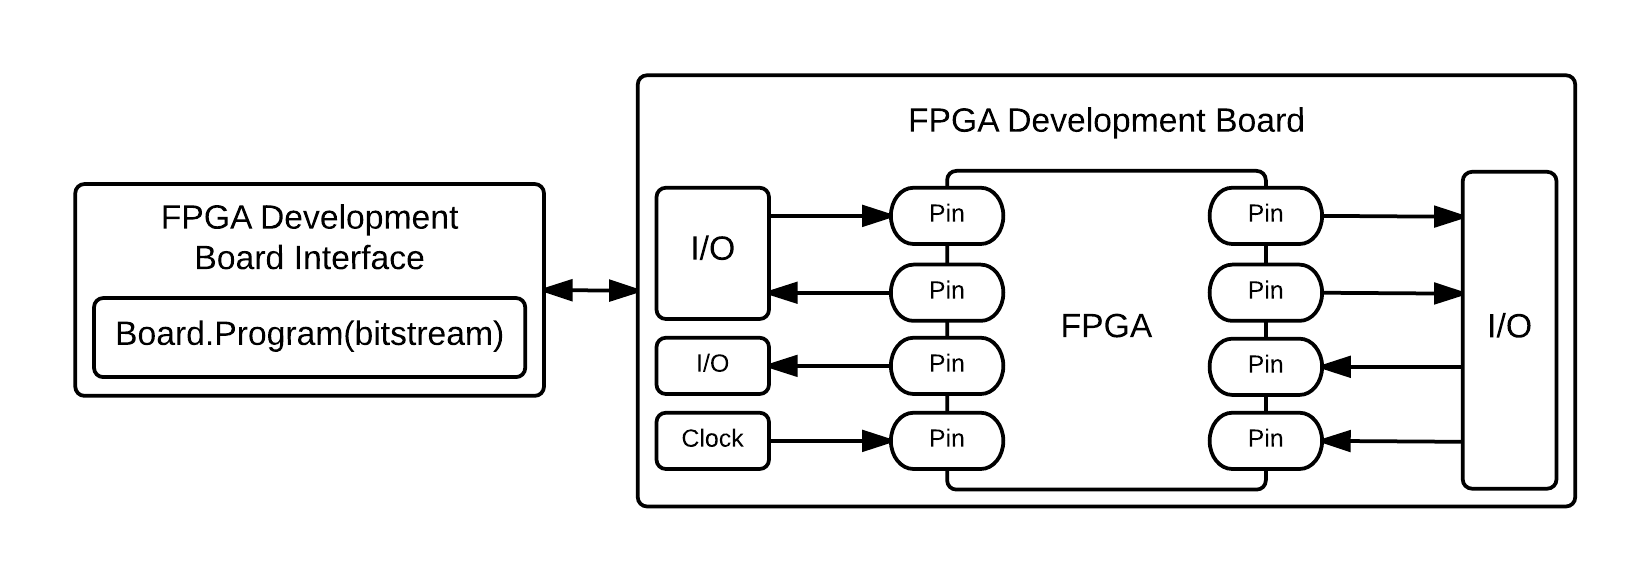
\includegraphics[width=0.8\textwidth]{img/overview-basic}
\end{figure}

In this basic model, the FPGA development board is considered to be a hosts for a FPGA and its various peripheral components. Not all pins of the FPGA's physical package and not all peripheral devices are considered to be relevant to the model. Only the pins whose signals can be controlled through the FPGA's contained logic are included. Peripheral devices that do not connect to these pins, such as power supplies or programming circuits are excluded from the model. Specifically, the presence of a clock generating device is assumed, providing the FPGA with a clock signal on one of its pins. 

Besides the omission of details of the FPGA's peripherals, a part of the FPGA's internal complexities are hidden from the model as well. Figure \ref{fig:fpga-basic} gives a graphical overview of the FPGA's internals and its contained logic. The FPGA's internal interface is simplified and defined to be a container for the end product of a HDL developer's work: an entity with input signals, output signals and an input clock signal. Other physical, electrical or logical characteristics of the FPGA are not included in this model.

\begin{figure}[h]
    \centering
    \caption{The basic model, an overview of the FPGA and its contained experiment setup logic. No specific architecture is applied to the logic.}
    \label{fig:fpga-basic}
    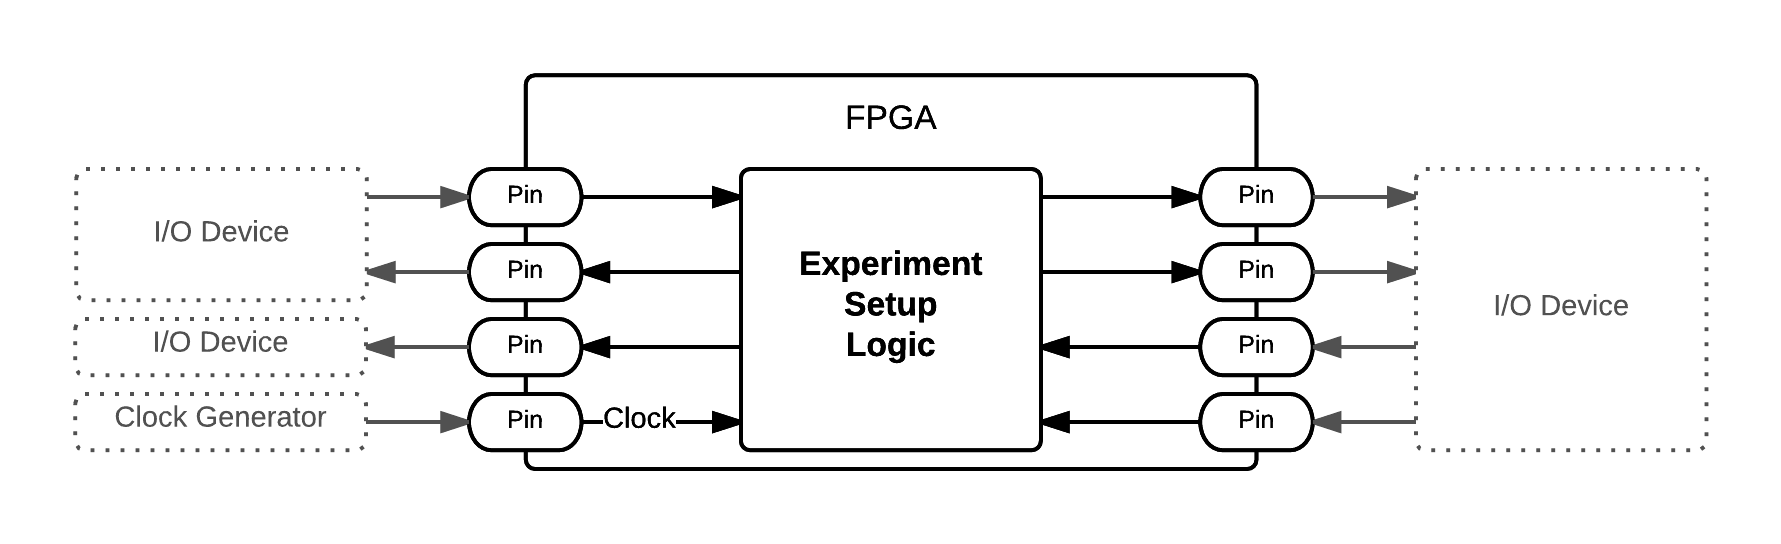
\includegraphics[width=\textwidth]{img/fpga-basic}
\end{figure}

In the case of this basic model, no specific architecture is defined that will embed the experiment setup logic into the FPGA development board. A specific architecture will be developed in the following stages. At this stage of the model, a developer is responsible for the development of its own architecture that embeds the experiment setup logic into the environment of the FPGA.

In this basic model, two user roles are defined: experiment setup developers and experimenters. In a classroom environment, an instructor can be considered an experiment setup developer and a student can be considered an experimenter. 

\subsection{Experiment Setup Development}
\label{sectionexperimentdevelopers}
Experiment setup developers are responsible for the design, implementation, testing, documentation and distribution of experiment setups for use on FPGA development boards. The end product of their work is a package containing a bitstream file and optionally the source files used in the bitstream file's compilation process. This package is referred to as an experimentation package. Figure \ref{fig:process-development-basic} displays a graphical overview of the experiment setup development process. 

\begin{figure}[h]
    \centering
    \caption{The basic model, an overview of the experiment setup development process.}
    \label{fig:process-development-basic}
    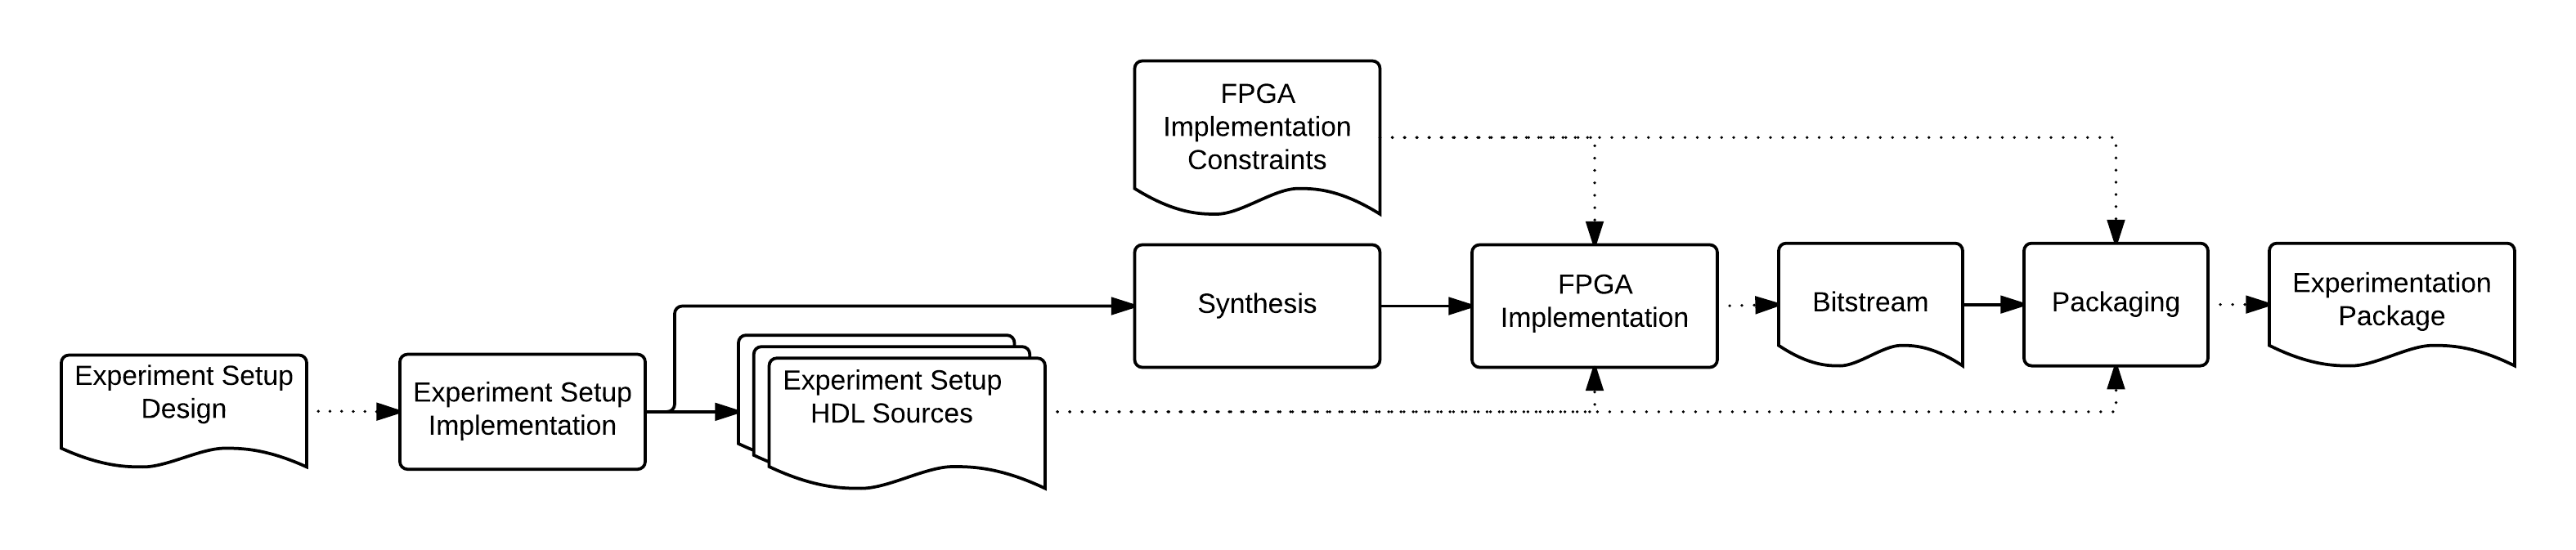
\includegraphics[width=\textwidth]{img/processes-basic-development}
\end{figure}


% TODO onderstaande opsomming is beter op zijn plaats in de problem statement.
% As shown below, an experiment setup developer must have knowledge of a significant number of subjects and technologies: 

% \begin{itemize}
% \item Designing an experiment setup requires knowledge on the subject of digital logic and digital systems. 
% \item For the design to contain meaningful educational content, the developer should have experience in teaching the subject. 
% \item Translating the design into a working, valid implementation in VHDL or Verilog requires experience in HDL development.
% \item Embedding the implemented design in a FPGA development board requires knowledge of the specific FPGA, its development tools and the FPGA's peripheral devices.
% \end{itemize}

\subsection{Experimentation}

Experimenters are responsible for carrying out experiments. They obtain experimentation packages and initialize experiment setups on their FPGA development boards. In order to complete the experiment, they make observations and interact with the experiment setup that is contained within the FPGA. Figure \ref{fig:process-experimentation-basic} displays a graphical overview of the experimentation process. In this basic model, two different methods of interaction are defined: interaction through board I/O devices and interaction through the process of HDL source modification, recompilation and reprogramming. Observation of the experiment's results can be done through the FPGA development board's I/O devices. Some development tools allow for live inspection of the FPGA's internal signal levels through a PC connection and specialized software.

\begin{figure}[h]
    \centering
    \caption{The basic model, an overview of the experimentation process.}
    \label{fig:process-experimentation-basic}
    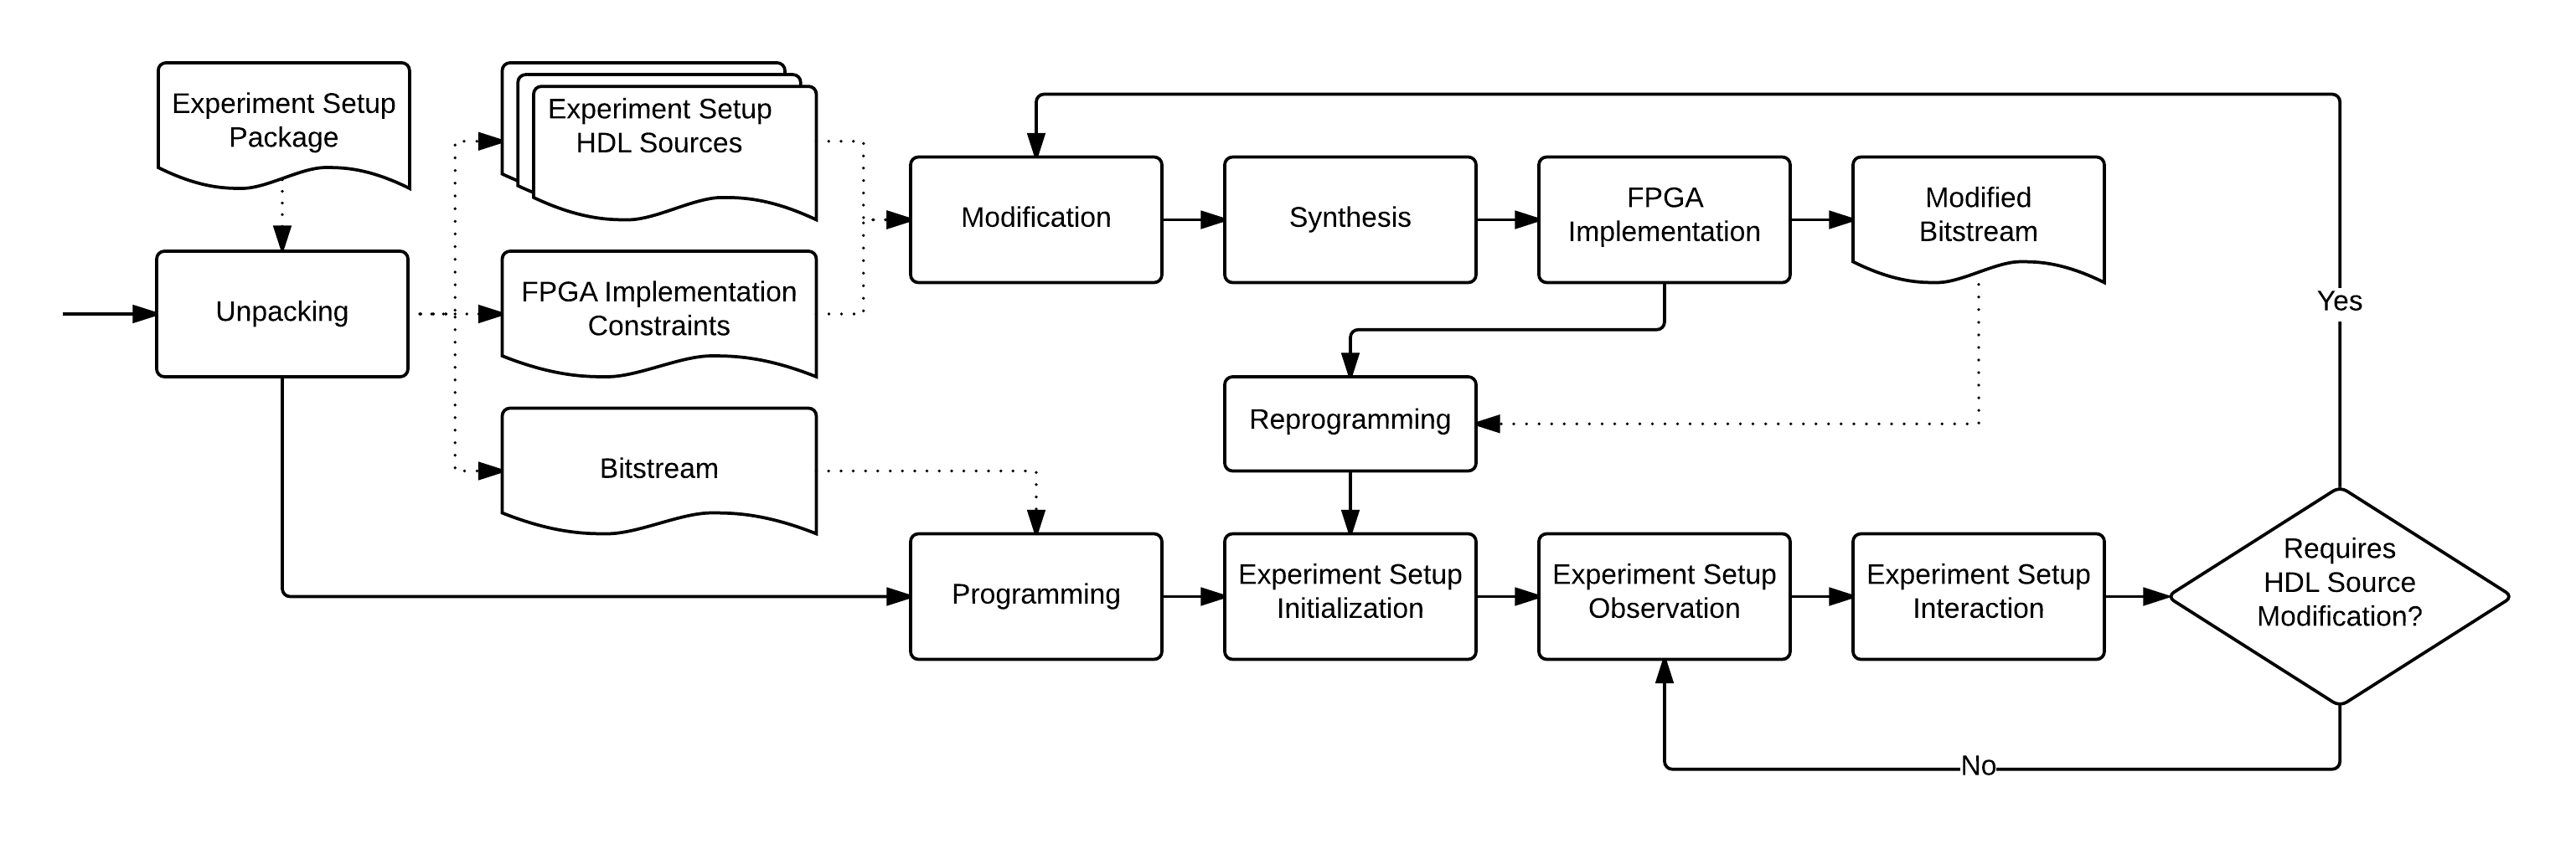
\includegraphics[width=\textwidth]{img/processes-basic-experimentation}
\end{figure}

In order for a user to act as an experimenter, one must understand the logic and workings of the obtained experiment setup. Furthermore, an experimenter must understand the basic concepts and role of the FPGA development board, as well as how to program the FPGA via the experimenter's PC. In preparation of the experiment, experimenters must install programming software and operating system drivers for the FPGA development board. In this case, interaction and observation is done through the board's I/O devices. 

Including the PC as a tool for observation and interaction requires additional knowledge and preparation from experimenters. In order to understand and modify the experiment setup's HDL sources, users must be familiar with the programming language used. Recompilation requires users to install and understand the FPGA's development tools in order to set up a proper development environment. Furthermore, this method of interaction will significantly increase the time required for every change to be processed, since the process of recompilation is a time consuming process. Using the FPGA as a tool for observation requires further familiarization with the FPGA's development tools.

\section{Virtualizing I/O}
\label{sectionvirtualizingio}

% TODO In deze sectie verduidelijken dat state control nog niet mogelijk is en dat interne state alleen inzichtelijk kan worden gemaakt door expliciet signalen naar buiten te brengen in het experiment ontwerp.

% TODO Er wordt een externe user interface gepresenteerd als oplossing. Hoe ziet deze er uit?

% TODO: Toto: zijn er geen downsides van het gebruik van software?

Regular FPGA development boards offer a limited set of I/O devices. As a consequence, this allows for observation and control of experiment setup logic entities with a limited number of input and output signals. Embedding entities with a large number of inputs and outputs however, requires a different approach. 

In order to support experiment setup entities with a large number of input and output signals, the basic model's logic architecture is extended through introduction of the controller. Figure \ref{fig:fpga-inout} gives an overview of the FPGA and the newly defined architecture. The experiment setup entity's inputs and output signals are available to the controller only, but both components still share a common clock signal. The signal levels of the FPGA's peripheral devices are no longer driven by the experiment setup entity. Following the previous section's criteria, these devices are considered irrelevant and thus removed from the model. Only the clock generating device and a single machine-machine communication device remain part of the model. 


\begin{figure}[h]
\centering
\caption{I/O virtualized, an overview of the FPGA and its contained logic architecture. The controller embeds the experiment setup logic into the FPGA.}
\label{fig:fpga-inout}
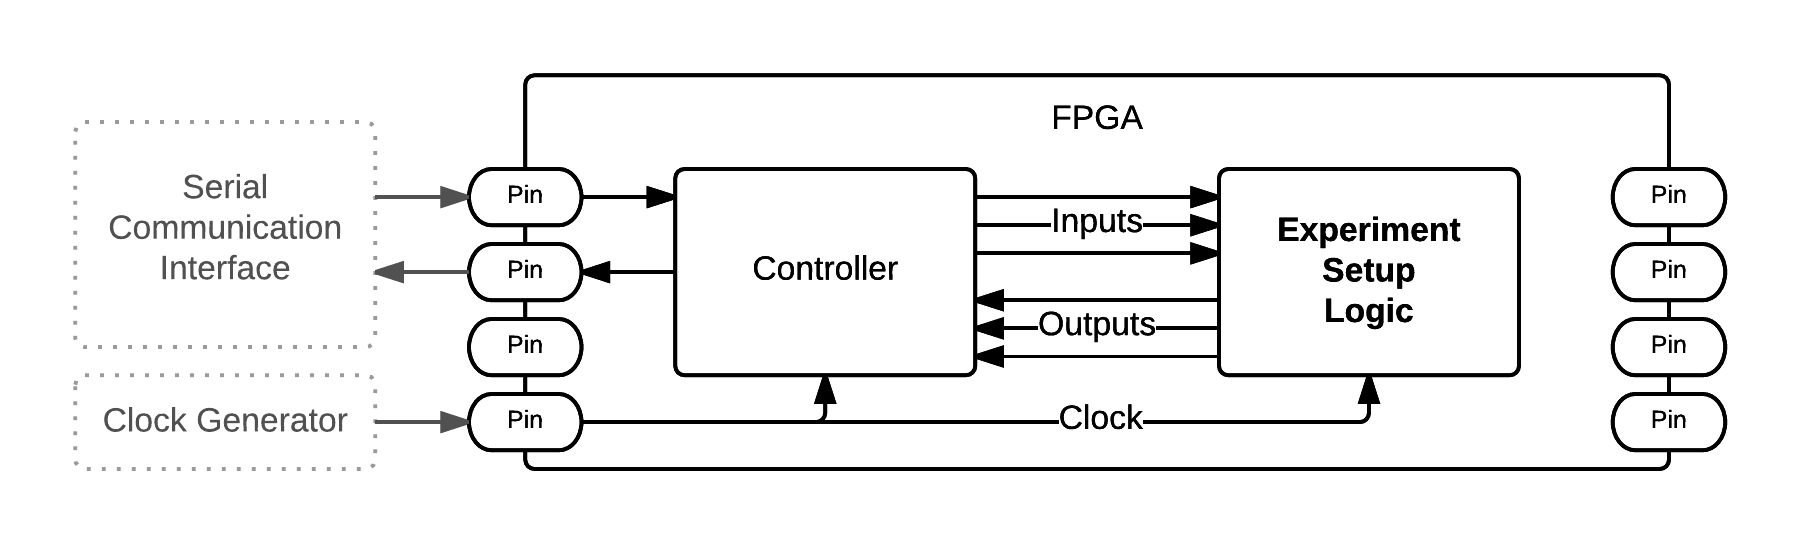
\includegraphics[width=\textwidth]{img/fpga-inout}
\end{figure}

% Concept controller ook te zien in \cite{jansen2014every}

The controller is defined to be a component that acts as an intermediary between the experiment setup logic and an experimenter's PC. The experiment setup's state is observed and controlled through controller-specific software, a method also presented in \cite{holland2003harnessing} and \cite{bulic2013fpga}. A hardware-based method to observe and control the experiment setup's state is described in \cite{al2007teaching}. A software-based solution however, allows for a flexible interface as well as a self-contained solution in terms of physical components. 

The controller exposes an additional interface through a communication channel that must be provided by one of the FPGA development board's communication devices, as can be seen in figure \ref{fig:overview-inout}. This interface defines operations that allow for the experiment setup entity's individual input and output signals to be controlled and observed respectively. A similar interface for observation and control of specific signals is described in \cite{holland2003harnessing}. 

\begin{figure}[h]
\centering
\caption{I/O virtualized, an overview of the FPGA development board and its exposed interfaces.}
\label{fig:overview-inout}
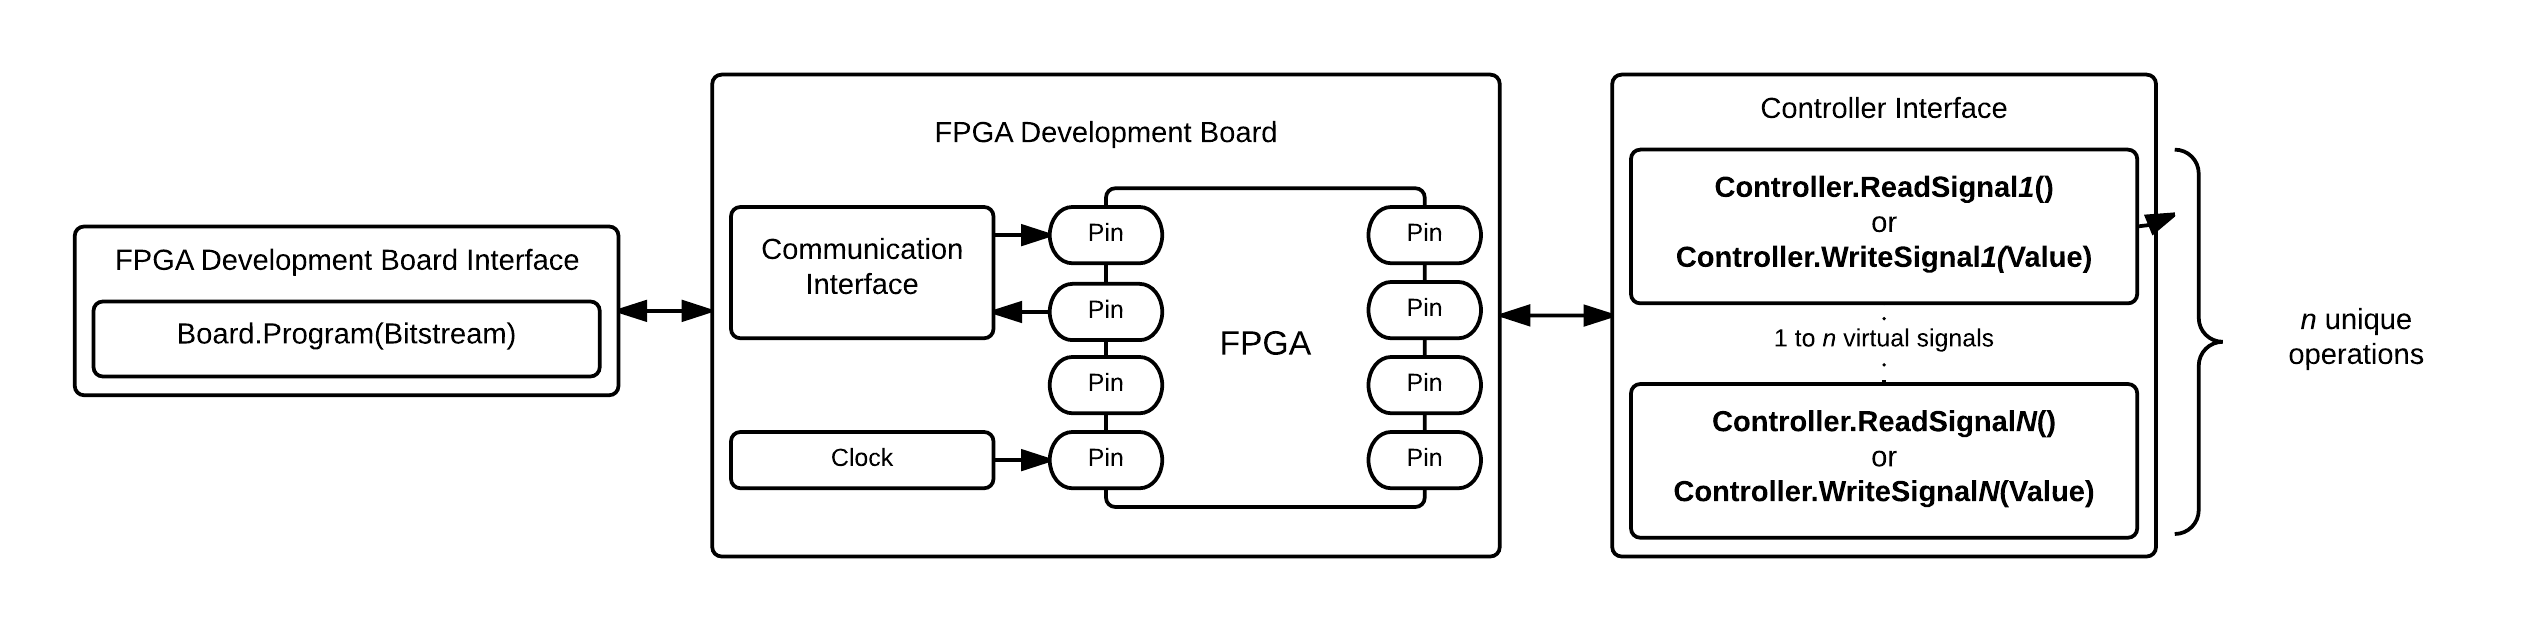
\includegraphics[width=\textwidth]{img/overview-inout}
\end{figure}

The explicit separation of concerns in the logic architecture allows for separate implementation and validation processes for experiment setup logic, controller logic and PC software. This partitioning subsequently allows for distribution of work among specialists, removing the need for a single experiment developer to have knowledge and experience in all the areas previously described in section  \ref{sectionexperimentdevelopers}. As a consequence of the separation however, more dependencies are introduced into the development process. The development of a controller component requires a definition of the experiment setup's interface and any change in this interface definition requires modification of the controller. A similar dependency exists between the controller and the PC software. A change in the experiment setup entity's interface definition will thus not only result in the need for modification of the controller, but in the need for modification of the PC software as well. These dependencies are addressed and removed from the model in section \ref{sectioncontrollerabstraction}.

Experiment setup interaction through dedicated PC software will simplify the experimentation process for experiment setups with large number of input and output signals. Involving the PC removes the need for experimenters to install and familiarize themselves with the FPGA's development tools. Experimenters will be able to interact with the experiment setup through a graphical interface on the PC, removing the need need for HDL programming skills and allowing for real-time interaction, since no recompilation is required. Since the board's I/O devices have been removed at this stage of the model, there is no possibility for users to physically interact with the experiment. The PC software provides the only means of interaction with the experiment setup.


\section{Cycle control}

% TODO: Taco: Toch eens onderzoeken wat voor mogelijkheden clock domains bieden, mogelijk beschrijven in chapter background.

% TODO: Timing diagram ter verduidelijking clock_enable

\label{sectioncyclecontrol}
% In the previous section, the basic model has been extended to include a definition of the controller. This controller allows for the embedding of experiment setup entities with an arbitrary number of input and output signals that are defined through combinational logic. 

The availability of a clock signal in the current model does provide support for experiment setup entities that are defined through synchronous sequential logic. At this stage of the model's development however, this clock signal is constant and cannot be varied in speed or stopped temporarily. Embedding an experiment setup entity of synchronous sequential logic would result in an uncontrollable situation of continuous state changes at high speed. In order to be capable of cycle-accurate observations and control over synchronous sequential experiment setup logic, the model requires further extension.

\begin{figure}[h]
\centering
\caption{Cycle control, an overview of the FPGA and its contained logic architecture. The \texttt{Experiment Clock} and \texttt{Reset} signals are added to allow for cycle-accurate interaction and (re)initialization.}
\label{fig:fpga-control}
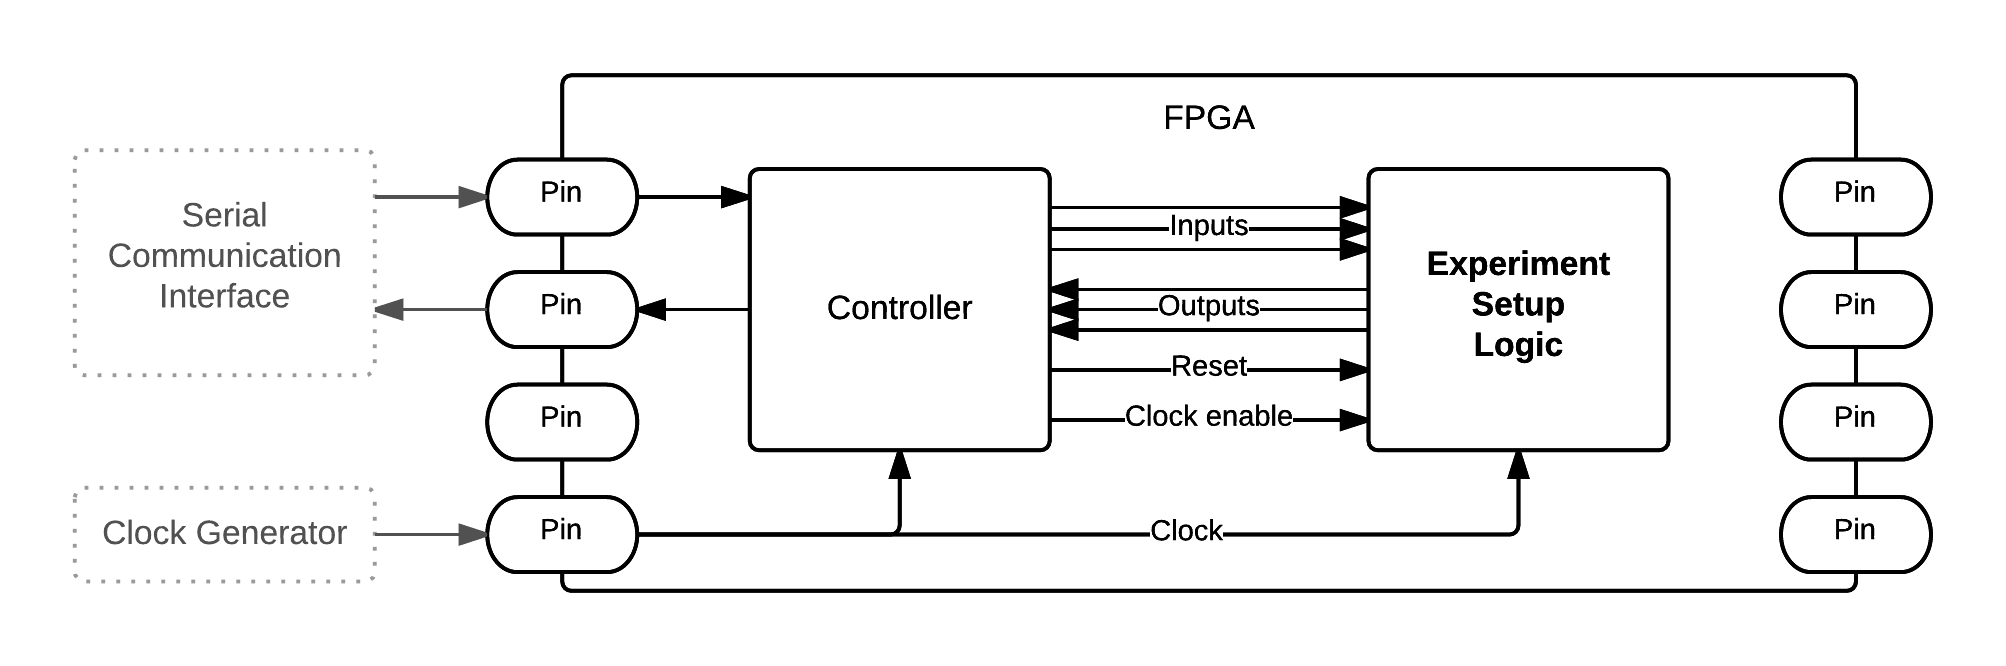
\includegraphics[width=\textwidth]{img/fpga-control}
\end{figure}

As a solution to the problem stated above, the FPGA's contained logic architecture has been extended, as displayed in figure \ref{fig:fpga-control}. The most significant change is the addition of the \texttt{Experiment Clock} input signal on the experiment setup's interface definition. As described in section \ref{section-fpga-clocking-resources}, a FPGA's clock delivery network generally contains buffers that allow for gating of clock signals. Utilizing this functionality in the controller's implementation will allow for the synthesis of a clock signal with pulses on irregular intervals. Combined with the \texttt{Reset} signal, these new input signals allow for cycle-accurate controlling and reinitialization of synchronous sequential logic contained within the experiment setup's logic.

% The introduction of the \texttt{clock\_enable} signal will require modification of every synchronous memory element present in the experiment setup logic, as displayed in figure \ref{fig:clock-manipulation-enable}. By multiplexing the input signal for every memory element based on the same \texttt{clock\_enable}, one can control the state change in a cycle-accurate manner. The method of using enable signals to control synchronous logic is described in \cite[Sec 2.4.5]{arora2011art}.

% One may argue that this approach is unfavourable, since it requires modification of existing experiment setup logic designs. This method for controlling state change however, is a common approach in FPGA-targeted HDL development and is used in many designs. More specifically, this approach was also taken in controlling the experiment setups described in \cite{holland2003harnessing} and \cite{bulic2013fpga}. As stated before, FPGAs do not allow for dynamic manipulation of clock signals by design, a method known as clock gating (figure \ref{fig:clock-manipulation-gated} ). Clock signals are distributed over the FPGA through dedicated lines that cannot be altered through HDL logic. Some manufacturers include support for static clock division, but still only down to relatively high speeds and do not allow for dynamic adjustment of clock speed [TODO: Bron]. 

% TODO: Opmerking Taco 
% Opmerking bij fig 3.8 discussie. Het board dat je gebruikt is een artix7
% en die familie (d.w.z. de "7" familie van xilinx) gedraagt zich anders. Er kunnen verschillende clockdomeinen gebruikt worden en dan
% heb je wel degelijk een soort van gated clock, hoewel dat nooit gebeurt via clk_gated = clk_org &
% enable. Lees het 7 series fpga clocking resources user guide document van xilinx!

% TODO: Toto: Meer uitleg bij deze figuren

% \begin{figure}[h]
%     \centering
%     \caption{Controlling state transitions through a clock enable signal and a gated clock signal.}
%     \label{fig:clock-manipulation}
%     \begin{subfigure}[t]{0.5\textwidth}
%         \centering
%         \caption{Gated clocks}
%         \label{fig:clock-manipulation-gated}
%         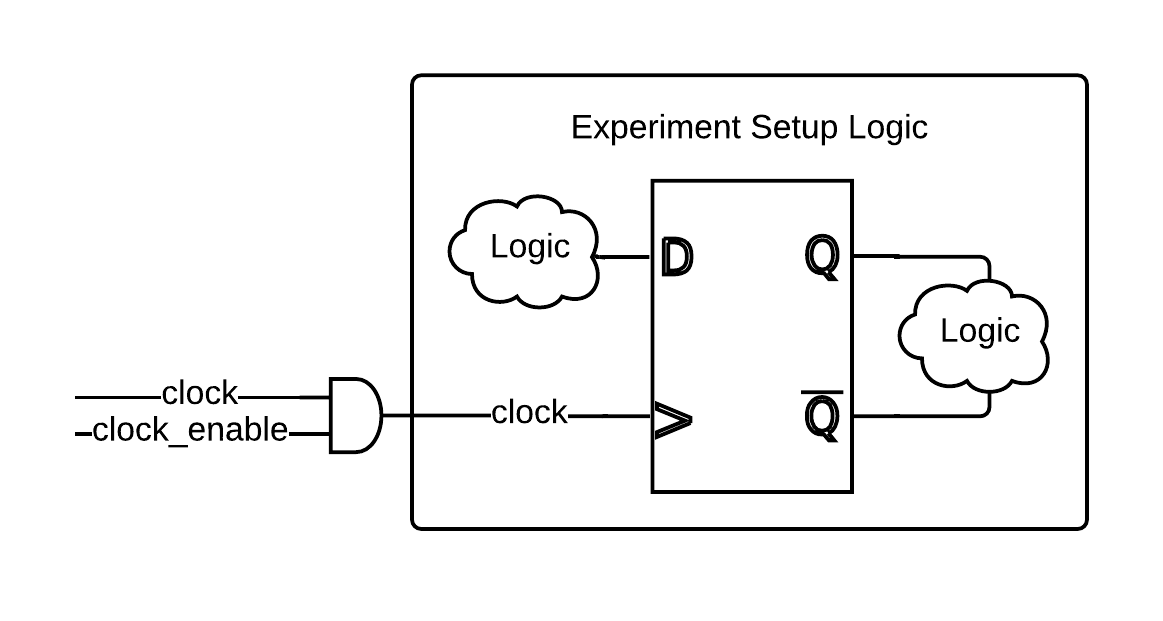
\includegraphics[height=1.5in]{img/clock-manipulation-gated}
%     \end{subfigure}%
%     \begin{subfigure}[t]{0.5\textwidth}
%         \centering
%         \caption{Enable signal}
%         \label{fig:clock-manipulation-enable}
%         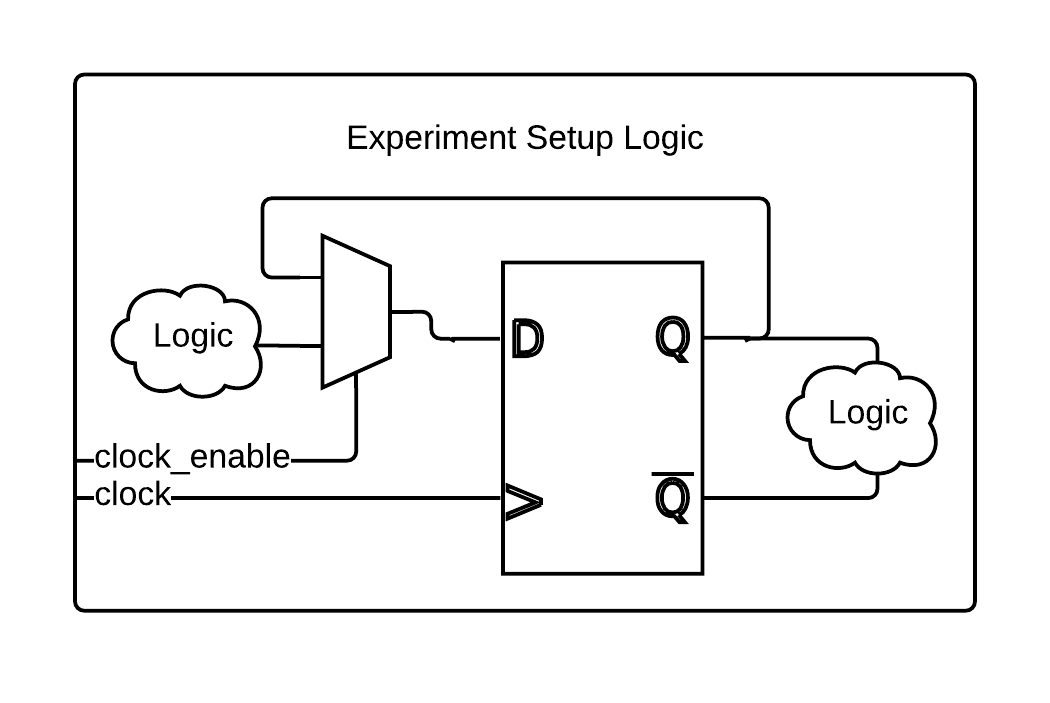
\includegraphics[height=1.5in]{img/clock-manipulation-enable}
%     \end{subfigure}%
% \end{figure}

\begin{figure}[h!]
\centering
\caption{Cycle control, an overview of the FPGA development board. The controller's interface is extended with operations that allow for cycle-accurate operation of the experiment setup.}
\label{fig:overview-control}
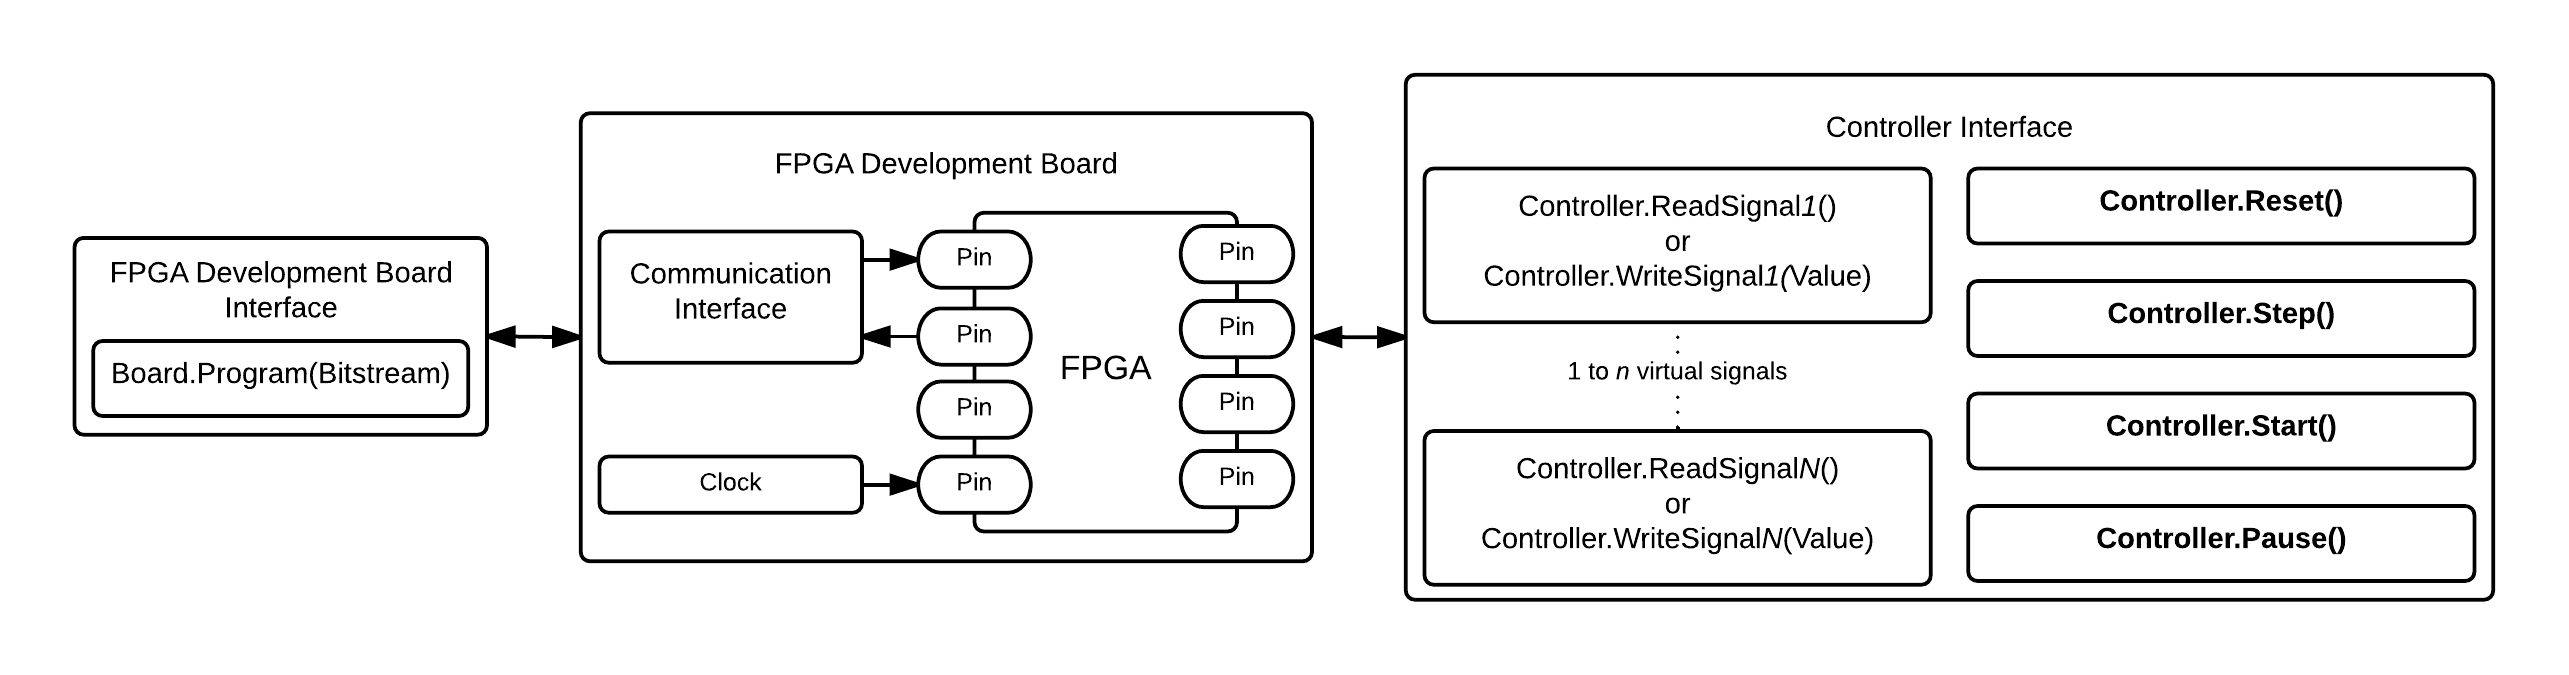
\includegraphics[width=\textwidth]{img/overview-control}
\end{figure}

In order to make this newly developed functionality available to the experimenter through the PC connection, the controller's interface is extended to support new operations that allow for the control of cycles. As displayed in figure \ref{fig:overview-control}, four new operations are available through the controller's interface. The \texttt{Controller.Reset()} operation (re)initializes the experiment setup to it initial state and waits for the next operation. Experimenters have manual control over the experiment setup's cycles through the \texttt{Controller.Step()} operation. The controller may also be instructed to manage the experiment setup autonomously through the \texttt{Controller.Start()} operation. The \texttt{Controller.Pause()} operation stops the controller's autonomous management of the experiment setup and awaits the next operation. Similar interfaces for cycle-accurate control of experiment setups are described in \cite{holland2003harnessing} and \cite{bulic2013fpga}.


\section{Experiment Setup Interface Generalization}
\label{sectioncontrollerabstraction}

% TODO: Taco: Hoe ga je de inhoud van complexe memory devices inzichtelijk maken?

% TODO: Taco: Wordt de experiment setup adapter gegenereerd?

% TODO: Taco gaat er van uit dat de experiment setup adapter de top component is.

% TODO: Taco: Uiteindelijke functionele omschrijving controller ontbreekt nog

% At this stage of the model's development, it supports the embedding of experiment setups defined through combinational logic as well as synchronous sequential logic. Experimenters can interact with these experiment setups through PC software that is specifically developed for the experiment setup. 
While the model has developed to address a number of problems encountered by experimenters, the problems experienced during development have only been partially addressed and tight coupling between logic architecture's components is still present. The source of these dependencies is the interface between controller and experiment setup logic, since every experiment setup has a unique interface. Through the establishment of a generic definition for the interface between experiment setup logic and the controller, this dependency is removed, allowing for reuse of board-specific logic in the development of different experimentation packages. 

\subsection{Address Space}
This thesis proposes an address space as a means of interaction with an experiment setup's input and output signals. More specifically, an address space is defined to be a virtual array of uniquely-addressed memory slots of equal size, a model equal to that of a computer's memory. The address space features the \texttt{read(address)} and \texttt{write(address, value)} operations, allowing for interaction. The model of an address space was chosen due to its compatibility with the problem of providing a generic approach to interaction with a statefull element, as well as computer scientists' familiarity with this model of representing state. This abstraction removes the tight coupling that existed between the controller and the experiment setup, since the unique relation between these two components no longer exists.

In order for an address space's individual slot to correspond to specific input or output signals, the signals are projected onto the experiment setup's address space. Figure \ref{fig:signal-address-projection} displays an example of such a projection. As can be observed, all of the experiment setup's input and output signals are projected onto the address space, except for the \texttt{clock} and \texttt{reset} input signals, which are separately driven by the controller. Experiment setup signals whose width exceeds that of the address space's individual memory slots are spread over multiple slots, spanning multiple addresses. Every signal corresponds to at least one unique address.

\begin{figure}[h]
    \centering
    \caption{Signal projection for a 12-bit counter experiment setup. In this example, the data bus is defined to have a width of 8 bits and the address bus is defined to have a width of 2 bits, defining 4 addresses.}
    \label{fig:signal-address-projection}
    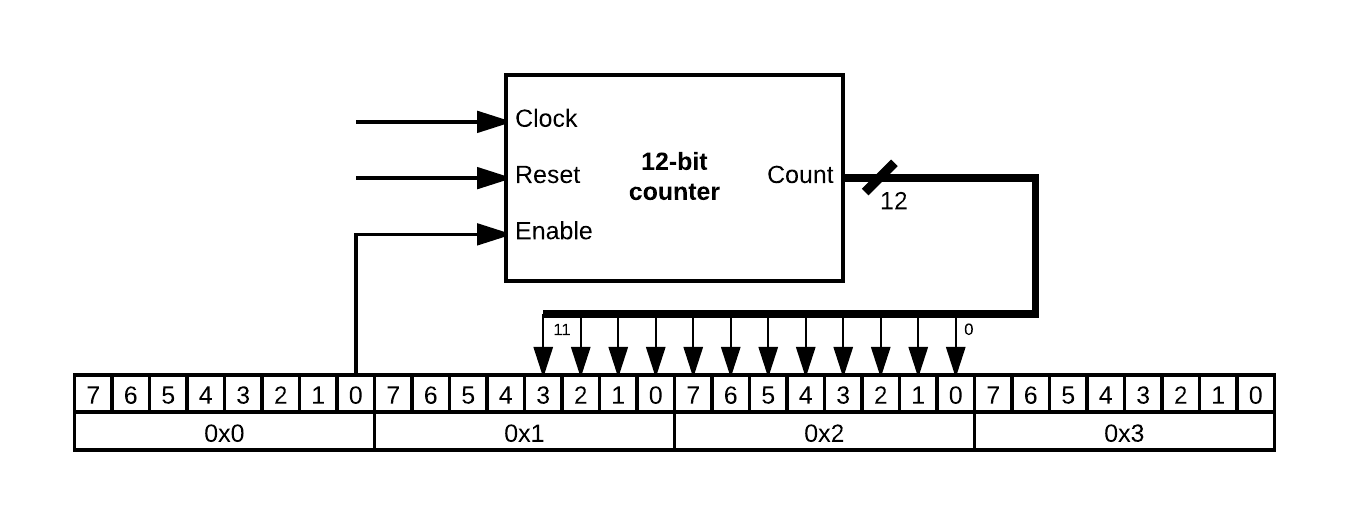
\includegraphics[width=0.8\textwidth]{img/signal-address-projection}
\end{figure}

As displayed in figure \ref{fig:fpga-abstract}, in addition to the experiment setup's primary logic, the logic architecture defines a secondary component that facilitates the projection of the experiment setup's signals on its address space. In order to allow for clear distinction between the different components, this new component is referred to as the experiment setup wrapper. The experiment setup wrapper has been given its name since it "wraps" around the experiment setup logic's input and output signals.  Additionally, the experiment setup's logic combined with this newly defined experiment setup wrapper is collectively referred to as the experiment setup component.

\begin{figure}[h]
\centering
\caption{Experiment setup interface generalization, an overview of the logic architecture contained within the FPGA.}
\label{fig:fpga-abstract}
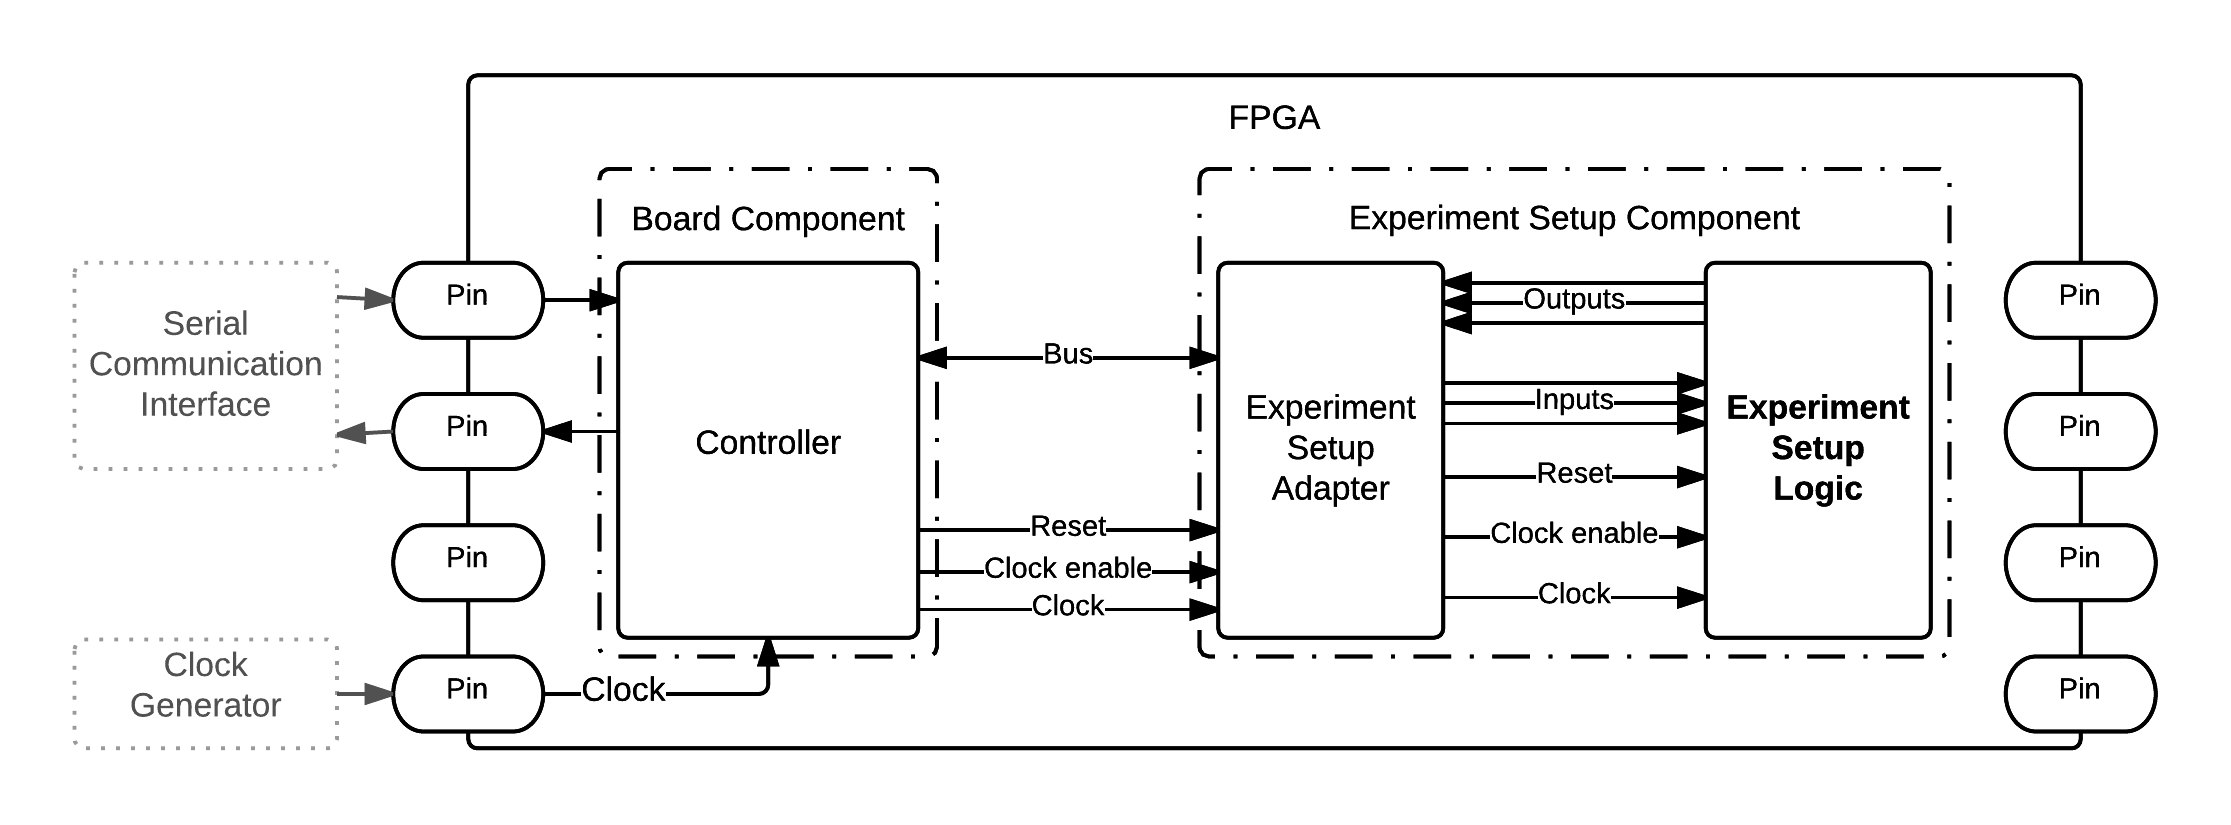
\includegraphics[width=.8\textwidth]{img/fpga-abstract}
\end{figure}

\subsection{Logic Interface}
In order to facilitate the address space abstraction, the experiment setup component's interface definition is modeled to resemble the interface of a simple block ram memory element. As displayed in figure \ref{fig:interfaces}, the experiment setup component's interface extends the block ram's interface with a \texttt{reset} input signal as well as an additional clock signal labeled \texttt{experiment clock}. This clock signal was introduced in the previous section for cycle-accurate control over the experiment setup logic. The second clock input labeled \texttt{clock} is a clock input whose signal is equal to that of the controller's. This clock signal allows for the operation of synchronous logic facilitating the address space projection.

\begin{figure}[h]
    \centering
    \caption{A comparison between the interfaces of a block ram and the experiment setup component.}
    \label{fig:interfaces}
    \begin{subfigure}[t]{0.5\textwidth}
        \centering
        \caption{Single-port block ram, derived from \cite[Ch.1]{ug473}.}
        \label{fig:interface-bram}
        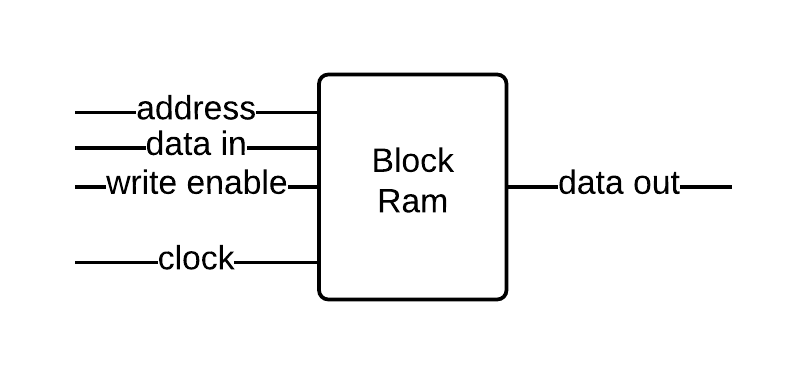
\includegraphics[height=1.2in]{img/interface-bram}
    \end{subfigure}%
    \begin{subfigure}[t]{0.5\textwidth}
        \centering
        \caption{Experiment setup component interface.}
        \label{fig:interface-experiment}
        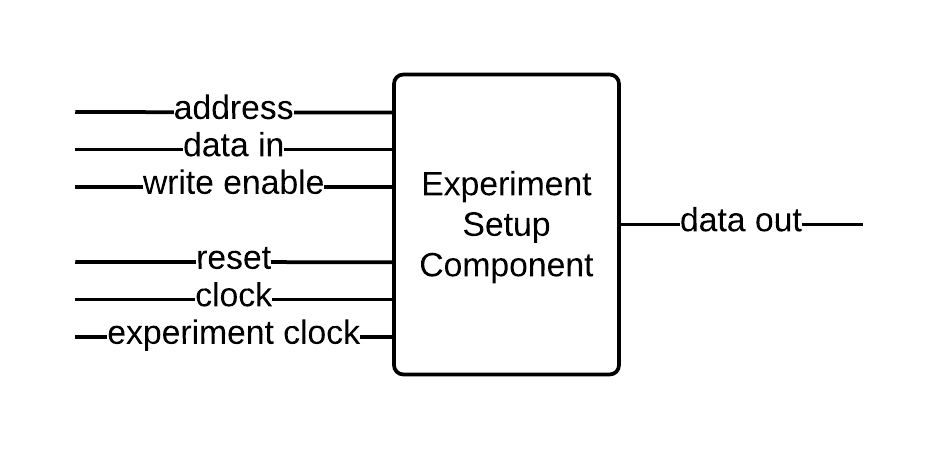
\includegraphics[height=1.2in]{img/interface-experiment}
    \end{subfigure}
\end{figure}

Additional to the similarities in interface signature, the experiment setup's interface is defined to have a behaviour similar to that of a block ram as well. Figure \ref{fig:timing-bram} displays a timing diagram that describes the experiment setup's signal behaviour for the \texttt{read()} and \texttt{write()} operations. Both operations are defined to take effect on rising clock edges, thus requiring the \texttt{data out} signal's levels to be buffered. 

\begin{figure}[h]
    \caption{Timing diagram for experiment setup logic, derived from \cite[Fig.1-2]{ug473}}
    \label{fig:timing-bram}
    \centering
    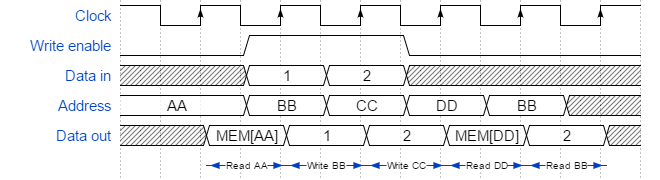
\includegraphics[width=0.85\textwidth]{img/timing-bram}
\end{figure}

\subsection{Generic Controller Interface}
A major advantage of the generic interface between the controller and the experiment setup component is that this can be directly translated into a generalization of the controller's command interface as well. As displayed in figure \ref{fig:overview-abstract}, the controller interface as exposed through the PC connection is modified such that the operations for signal interactions have been replaced by the \texttt{Controller.Read()} and \texttt{Controller.Write()} operations for interaction with the experiment setup component's address space. 

\begin{figure}[h]
\centering
\caption{Experiment setup interface generalization, an overview of the FPGA development board. The controller's interface no longer features direct control over specific experiment setup signal levels, but now features operations for interaction with the experiment setup's address space.}
\label{fig:overview-abstract}
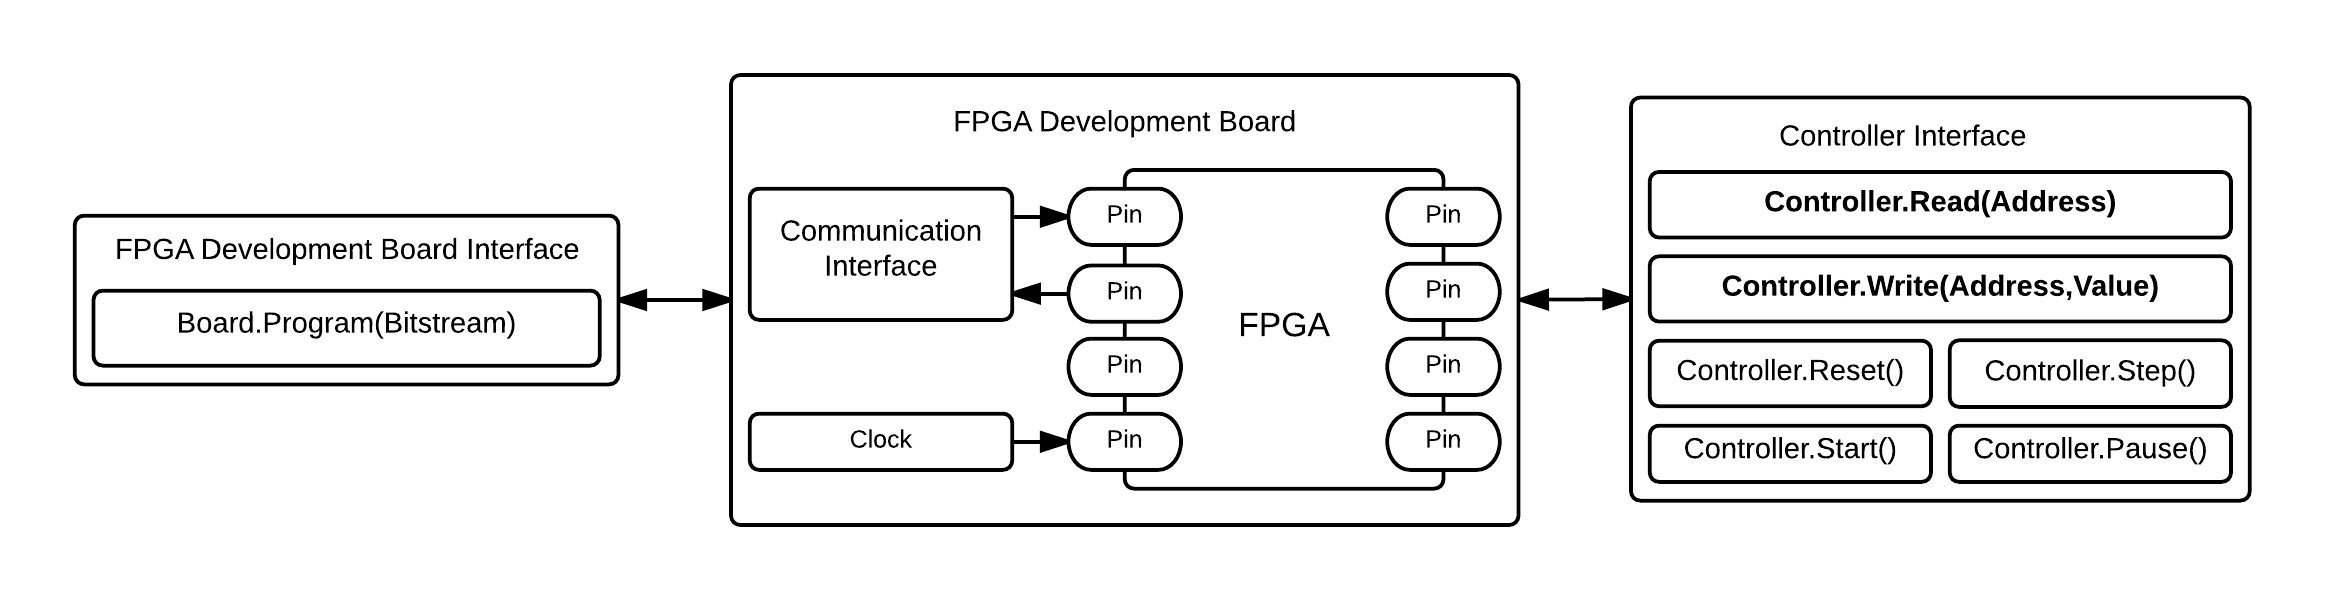
\includegraphics[width=\textwidth]{img/overview-abstract}
\end{figure}

Since the address space itself does not describe the experiment setup logic signals' projection, additional information is required for sensible interaction with the experiment setup component. The concept of an address space description is introduced, providing information about how the experiment setup's signals are projected on the experiment setup component's address space. 

\subsection{Processes}
Figure \ref{fig:processes-abstract-development} displays an overview of the process for the development of new experimentation packages. The experiment setup logic's HDL sources as well as the experiment setup wrapper's HDL sources are developed and composed to collectively define the experiment setup component's HDL sources. As part of the development of the experiment setup's wrapper, a description of the experiment setup's address space is created as well. 

The generalization of the experiment setup component interface allows for modification of the development process. It allows for independent development of board-specific controller logic HDL sources. The definition of a generic interface allows thus for these sources to be reused in the development of different experimentation packages. The comtroller's sources are combined with the experiment setup component's HDL sources in order to define the experimentation package's complete set of HDL sources. These sources can then be taken through the FPGA's compilation in order to generate a bitstream file. This bitstream file is then packaged with an description of the address space, in order to form an experimentation package.

\begin{figure}[h]
    \caption{ Experiment setup interface generalization, an overview of the experimentation package development process. The process allows for the reuse of controller HDL sources in the development of different experimentation packages.}
    \label{fig:processes-abstract-development}
    \centering
    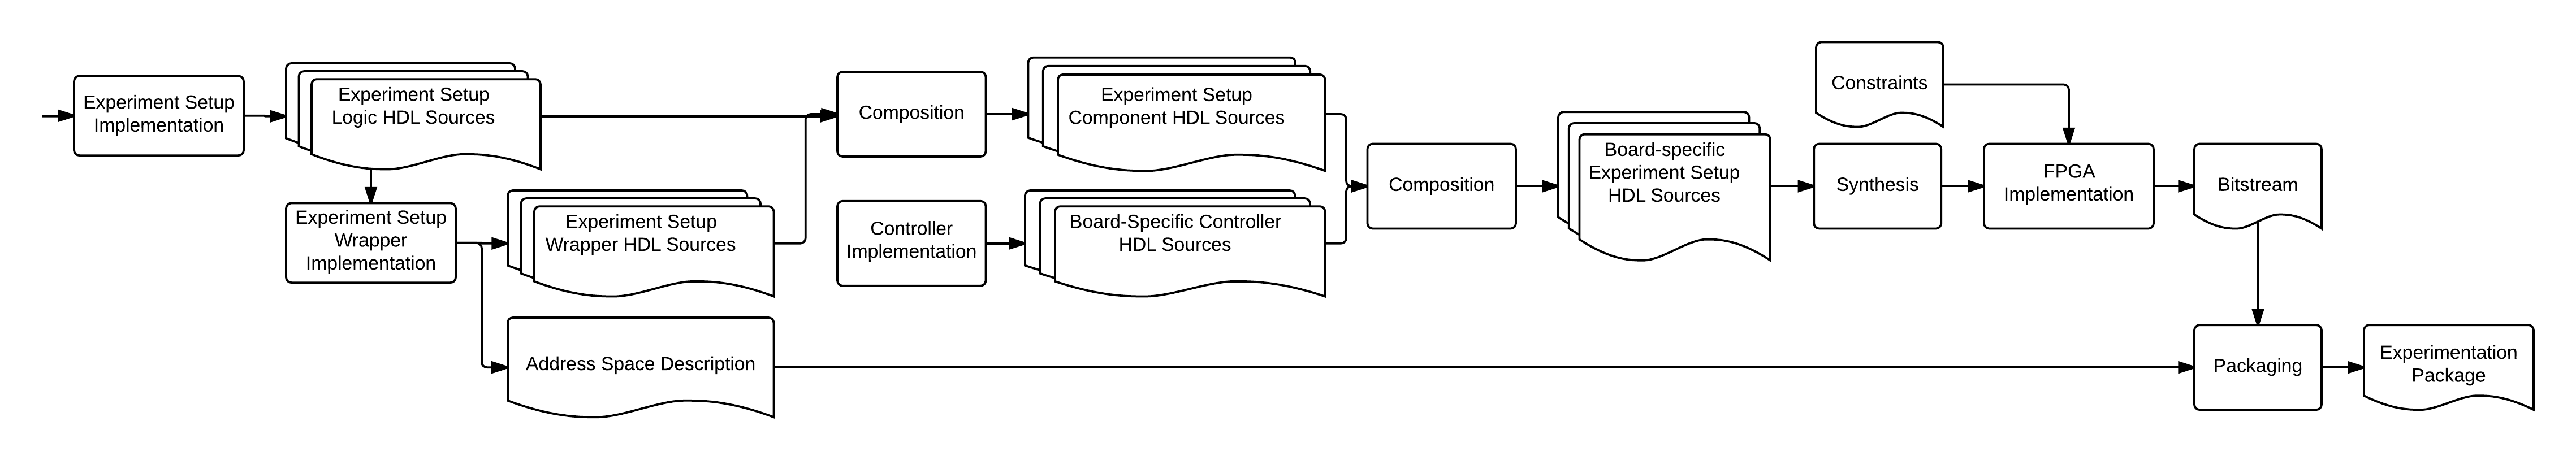
\includegraphics[width=\textwidth]{img/processes-abstract-development}
\end{figure}

The experimentation process as displayed in figure \ref{fig:processes-abstract-experimentation} is extended to include the experiment setup's address space description in the initialization of the exeriment setup, in order to allow for meaningful interpretation of the experiment setup's address space. 

\begin{figure}[h]
    \caption{ Experiment setup interface generalization, an overview of the experimentation process.}
    \label{fig:processes-abstract-experimentation}
    \centering
    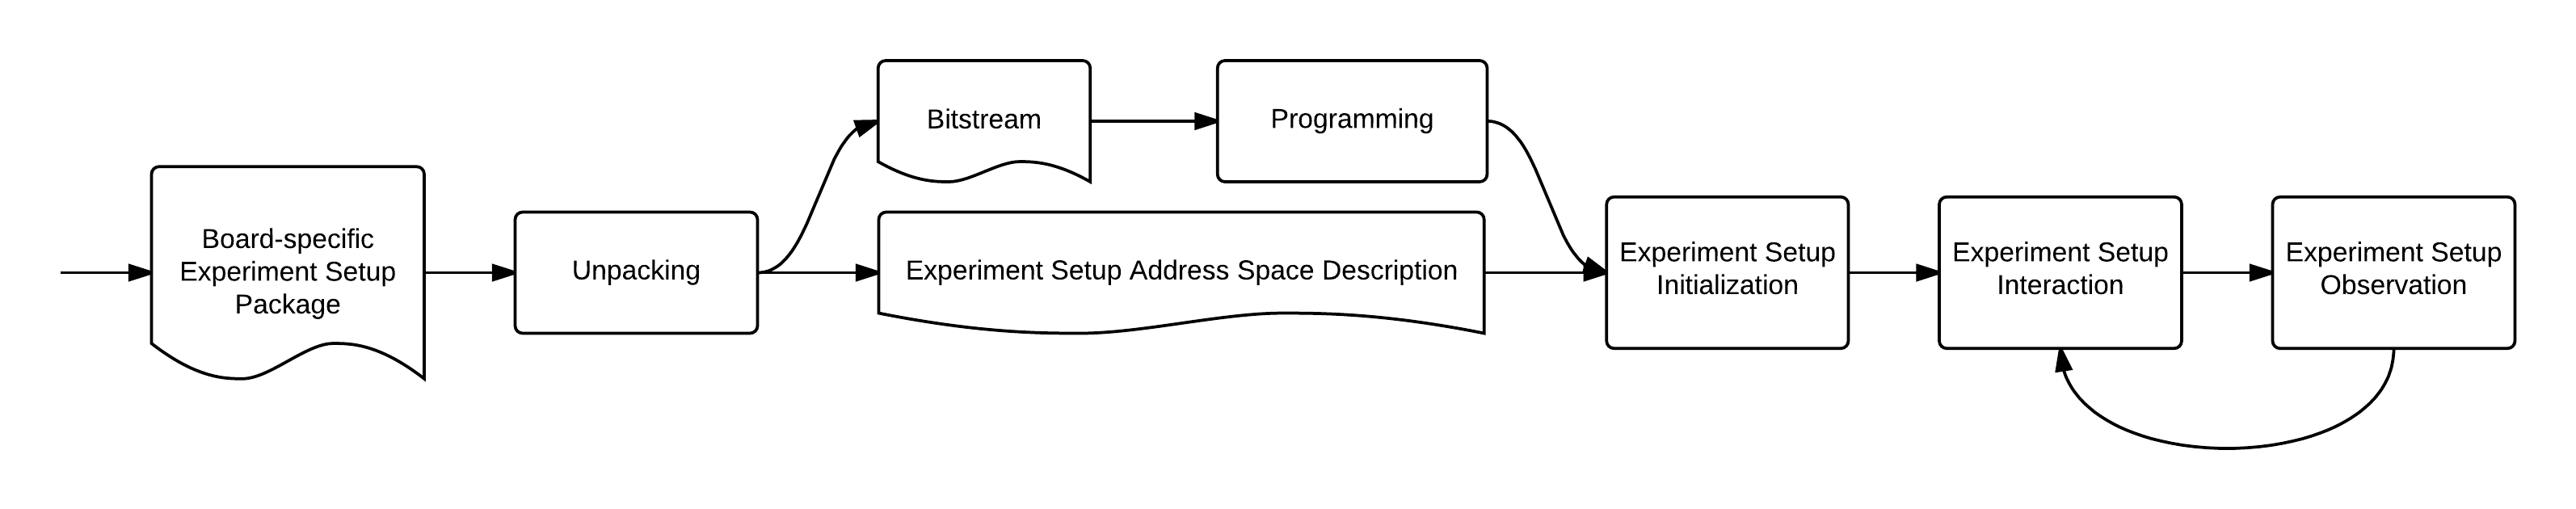
\includegraphics[width=\textwidth]{img/processes-abstract-experimentation}
\end{figure}


\section{Development Process Automation}
\label{sectiondevelopmentprocessabstraction}

Due to the previous section's modifications, the experimentation package development process has become more complex. In order to reduce the process' complexity, this thesis' model definition is extended with two new abstract operations that combine a significant part of the process' operations. Additional to reducing the experimentation package development process' complexity, these new abstract operations allow be executed in an automated fashion.

As displayed in figure \ref{fig:processes-abstract-automation-overview}, the experimentation package development process has been divided into three subsequent subprocesses: experiment setup logic development, experiment setup wrapping and the component composition. The detailed contents of these subprocesses are displayed in figure\ref{fig:processes-abstract-automation}. 

\begin{figure}[h]
    \caption{A high-level overview of the experimentation package development process. The process has been divided into three subprocesses in order to allow for automation.}
    \label{fig:processes-abstract-automation-overview}
    \centering
    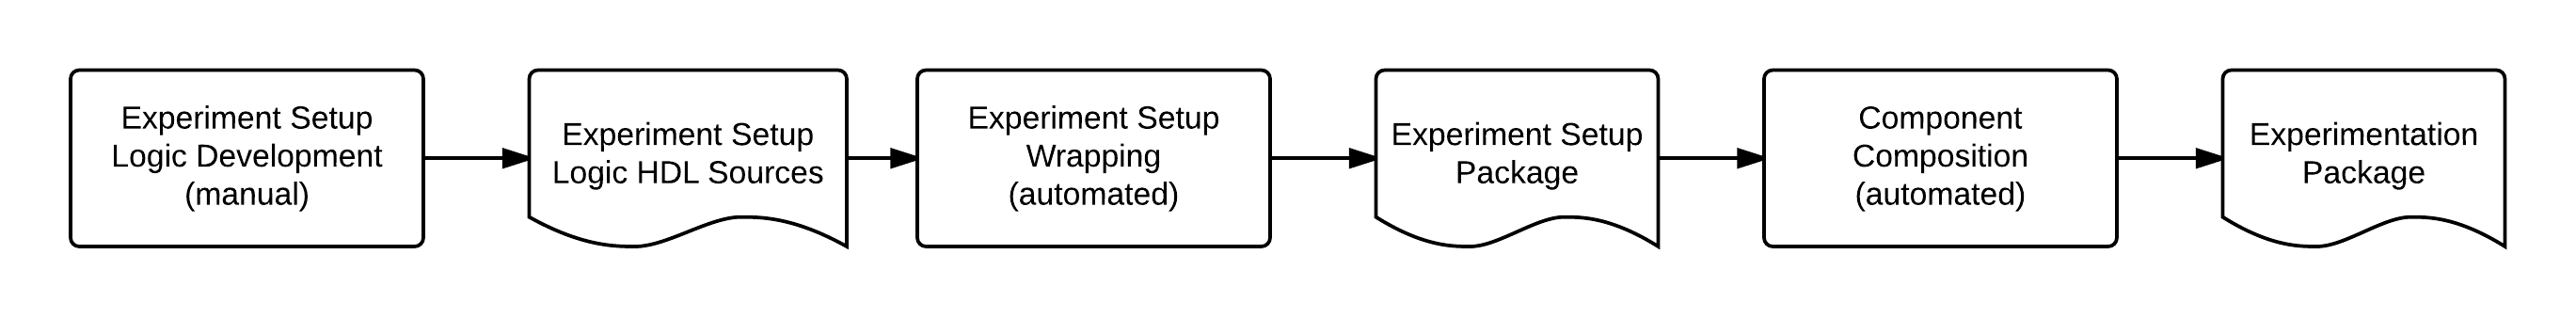
\includegraphics[width=\textwidth]{img/processes-abstract-automation-overview}
\end{figure}

\begin{figure}[h]
    \caption{A detailed overview of the experimentation package development process' subprocesses.}
    \label{fig:processes-abstract-automation}
    \centering
    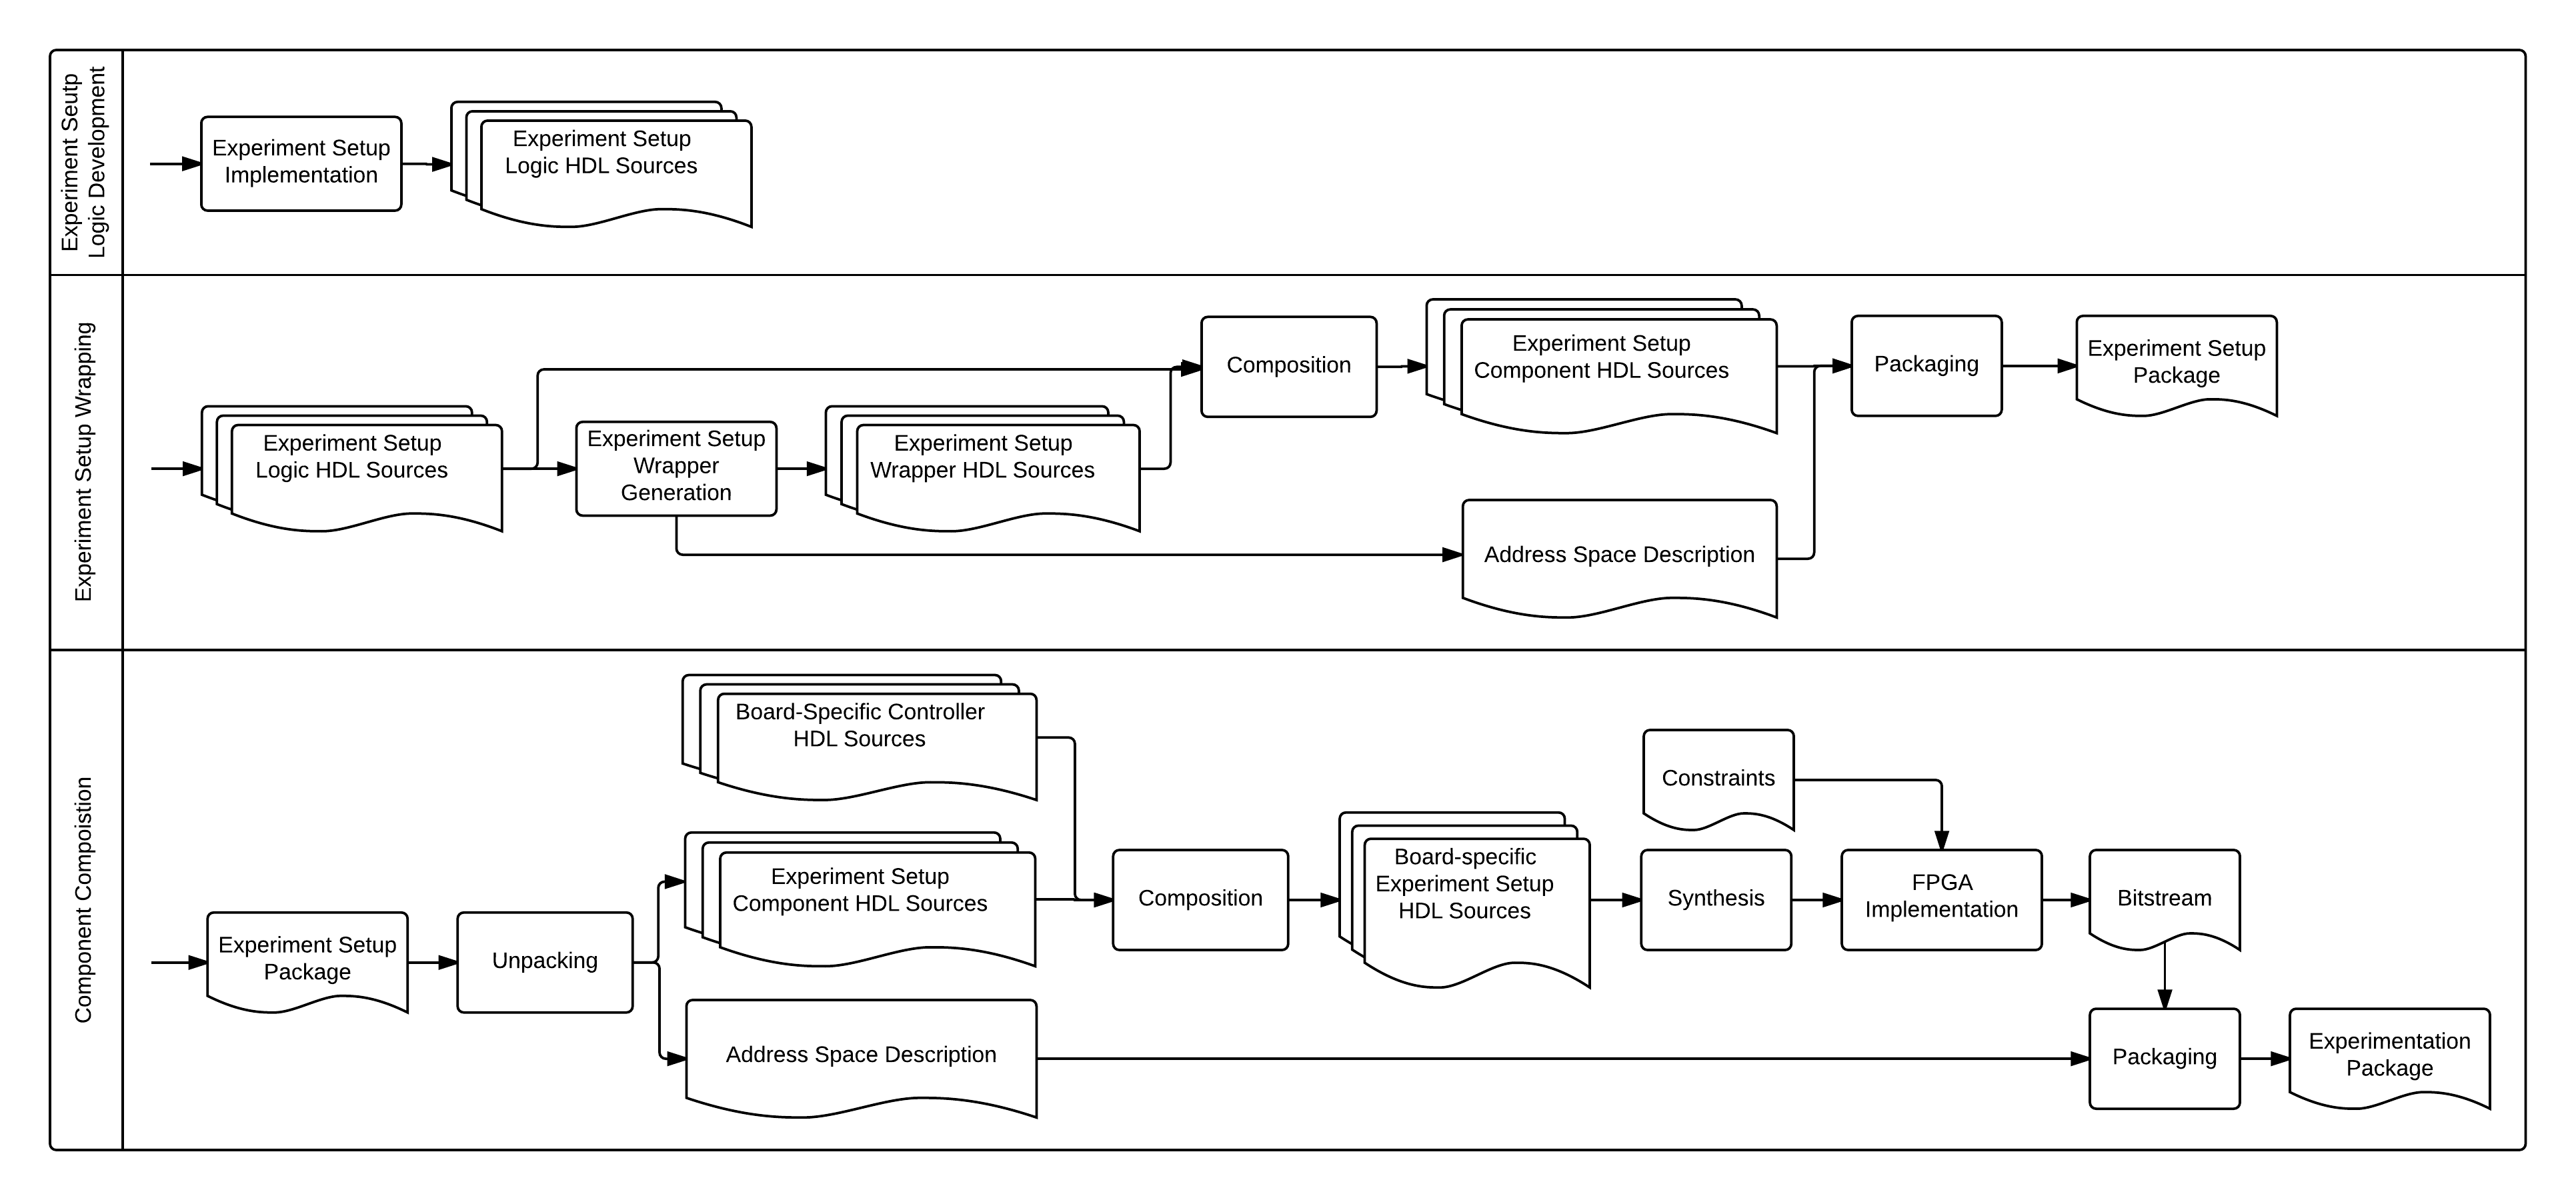
\includegraphics[width=\textwidth]{img/processes-abstract-automation}
\end{figure}

\subsection{Component Composition}
\label{sectioncomponentcomposition}
Since the board-specific controller sources can now be considered static across the development processes of different experimentation pacakges, a large part of the experimentation package development process' is composed of actions that are similar accross different projects. 

As an interface to this subprocess, the concept of an experiment setup package is introduced into the model's definition. This package acts as a unit of containment for the experiment setup component's HDL sources that was produced by the experiment setup wrapping process. Additional to the experiment setup's HDL sources, the package contains a description of the experiment setup's address space projection. This subprocess combines the user-defined sources from the input package with controller sources and processes these through the FPGA's toolchain. The resulting bitstream file is then pacakged into an experimentation package, together with the provided address space description.

The introduction of the component composition subprocess significantly reduces the complexity of the experimentation package development process. Due to the automated execution of its actions, these can be reduced to the abstract concept of component composition. The process abstracts the actions that relate to the FPGA and its toolchain, thus relieving the developer from the requirement of familiarizing itself with these tools and the related concepts.

\subsection{Experiment Setup Wrapping}
\label{sectionexperimentsetupwrapping}
The generalized interface between the experiment setup component's logic and the controller require users to adapt the experiment setup logic's interface through address space projection. This process of wrapping an experiment setup's logic may be automated through source code analysis and source code generation. The potential for automated execution of this subprocess further reduces the complexity of the experimentation package's development process. Through the abstraction of this subprocess' operations, the adaption of adapting experiment setup logic to match the model's generic interface is reduced to a single operation.

The experiment setup wrapping process as well as the component composition package are defined to be two separate processes. Although these subsequent processes may be combined into one automated operation, they have been defined as separate. In order to allow for advanced address space projections or wrapping logic that cannot be generated automatically, these processes have been defined as separate. 

% \subsection{Wrapping}
% The process of defining this experiment setup wrapping logic is thus named the "wrapping" process. As previously explained, this wrapper is composed of the logic that projects the experiment setup logic's input and output signals onto the experiment setup component's address space.

% A distiction can be made between experiment setup logic input and output signals, since both signals' levels can be determined through the address space \texttt{read()} operation, while only an input signal's level can be set through the address space's \texttt{write()} operation. \texttt{Write()} operations targeted at addresses on which an output signal has been projected have no effect. 

% Experiment setup input signals are driven by statefull elements contained within the experiment setup wrapper, whose signal level may be modified through a \texttt{write()} operation targeted at the corresponding address.

% The wrapping process can be automated, so even though it requires additional work from the experiment setup developer, but the 

% \subsection{Memory devices}
% %TODO sectie verbeteren, nog erg vage zinnen.

% The experiment setup has been considered to be an entity with input output signals. Any memory elements contained within the experiment setup can be made accessible through these input and output signals. This solution is not very scalable however. In order to allow for the controller to read and write to large memory elements such as block rams and register files, a different solution is required. A solution to this problem is displayed in figure \ref{fig:logic-wrap-extended}. 

% A simple wrapper can be computer-generated in many cases. If complex memory devices are contained within the experiment setup, a wrapper can be defined manually, using an experiment setup adapter component, address space splitters and memory interface multiplexers. 

% Large memory elements such as register files and block rams may be defined in HDL. During the compilation process, these elements are infered from HDL code and the FPGA's internal block rams are used. 

% If more memory space is required however, external memory devices such as DDR RAM IC's may be required. Since these external RAM devices require a number of cycles in order to accress the data, they must be abstracted in order to be accessible from within the experiment setup logic. In order to achieve the desired effect of seeing these DDR RAM devices as block ram devices that only require a single clock cycle to operate, the controller must stall the \texttt{clock\_enable} signal until the DDR controller finishes the desired operation. 

% iets zeggen over de faciliterende interface tussen PC en 




%variable address width
%variable data width

% studenten:
% - nog niet mogelijk snel te switchen
% docenten
% - afhankelijkheden tijdens ontwikkelproces.

% het is nog niet mogelijk te interfacen met complexe state devices in 

% Developed experiment setups are still board-specific

% Software is still controller-specific

% Controller-specific software

% Experiment-specific controller

% abstraction Allows for reuse of code

% abstraction allows for board-independent experiment development

% abstraction allows for random combination of experiment and controller, allowing for reuse of experiment code

% introduction of standard interfaces removes dependencies from development process

% Removing the dependency from controller to experiment, generic interface.

% Allows for reuse of generic board components for different experiment setup components.

% Complicates experiment development, but process of wrapping can be automated

% view of experiment as address space allows for easy interface from software address space allows for projection of signals as well as memory elements.









% \section{Reintroducing Board I/O}
% \label{sectionreintroducingio}

% Experiment setup has no accurate notion of time, so I/O devices can only be addressed as combinational devices. I/O device drivers facilitate this.

% Board I/O capabilities are of vital iportance in providing a physical hands-on experience. Although the FPGA itself is a physical object, the board's I/O capabilities expose the hardware setup's physical behaviour and provide real life interaction capabilities. Without this step, the whole point of a physical hands-on experience is lost.

% See figure \ref{fig:fpga-io}

% \subsection{I/O processing}
% Optionally, one needs to introduce device driver logic in order to allow for sequential I/O device logic to be usable as combinational logic. 




% \begin{figure}[h]
% \centering
% \caption{I/O reintroduced, overview}
% \label{fig:overview-io}
% 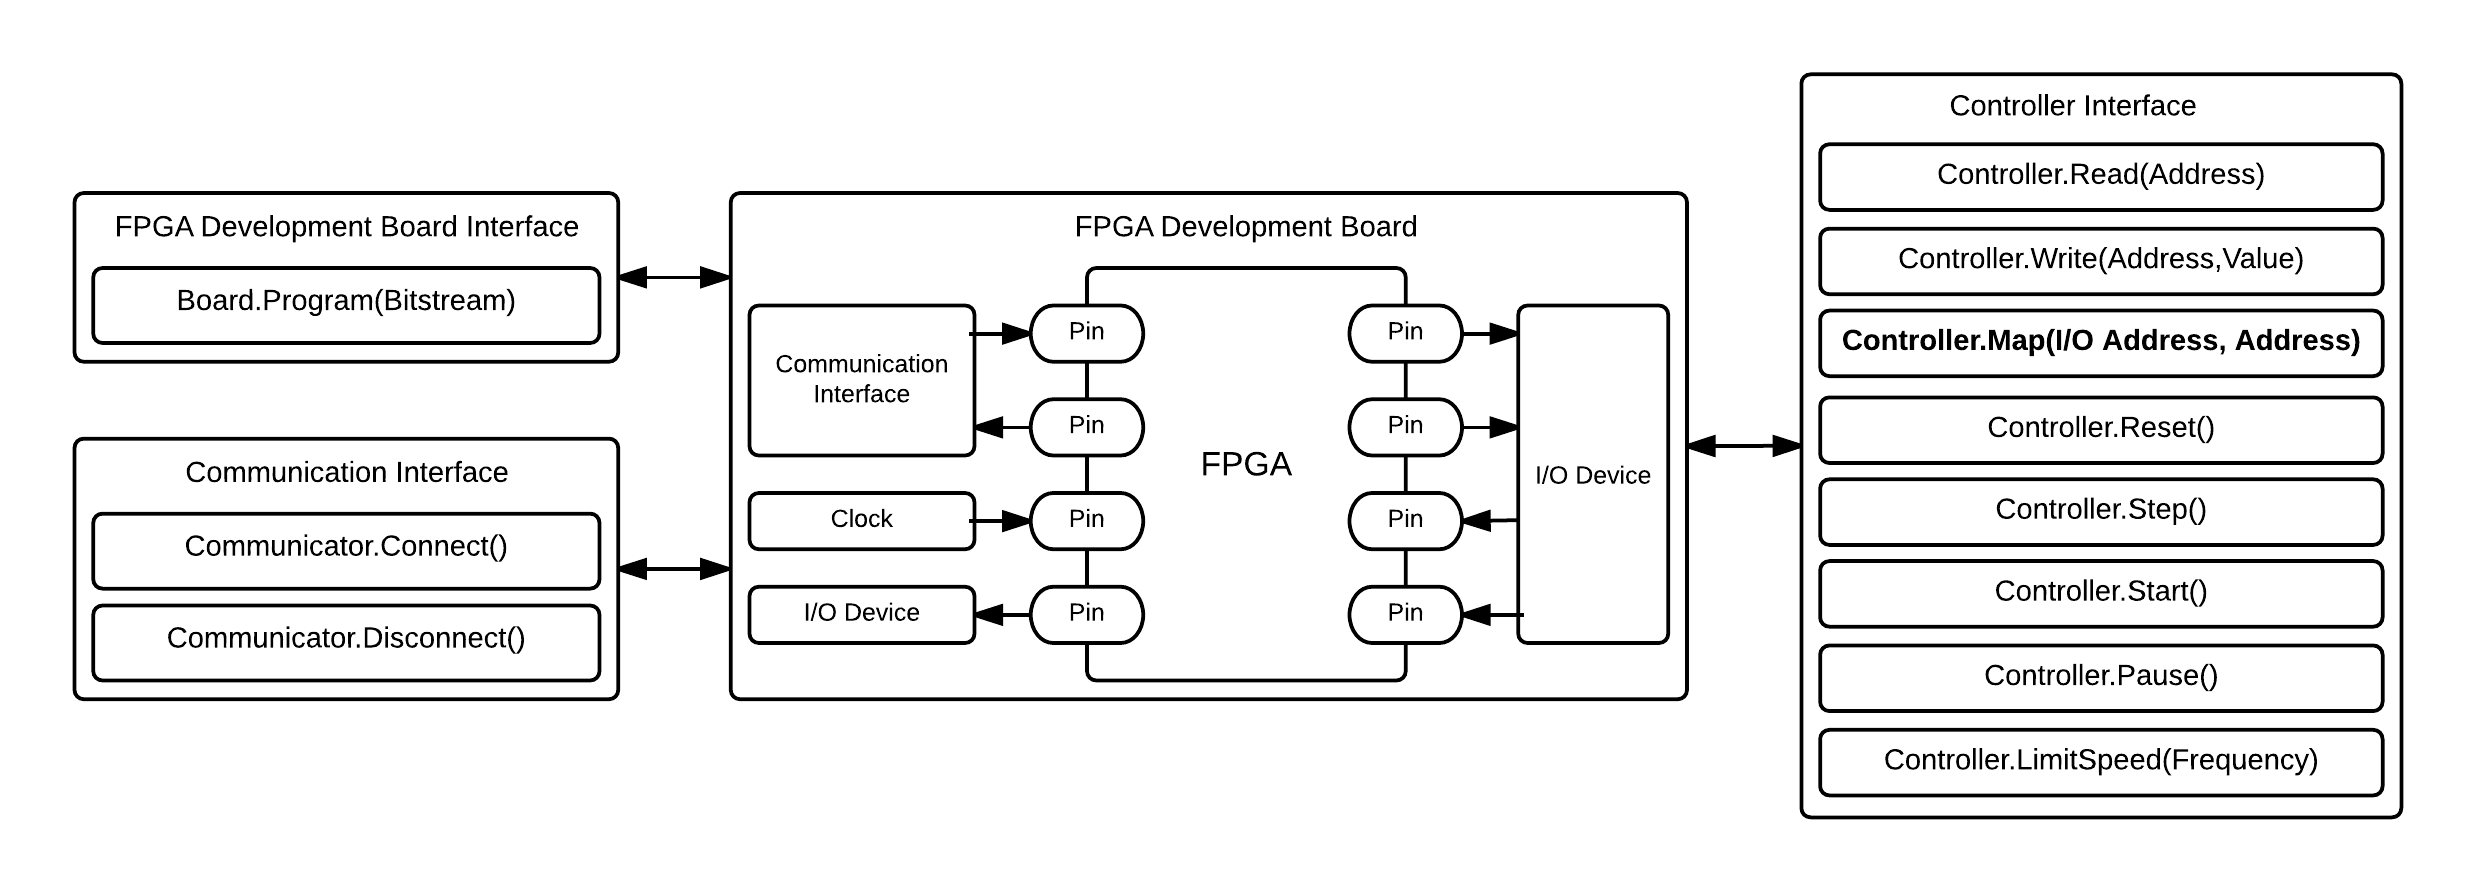
\includegraphics[width=\textwidth]{img/overview-io}
% \end{figure}


% \begin{figure}[h]
% \centering
% \caption{I/O reintroduced, FPGA logic design}
% \label{fig:fpga-io}
% 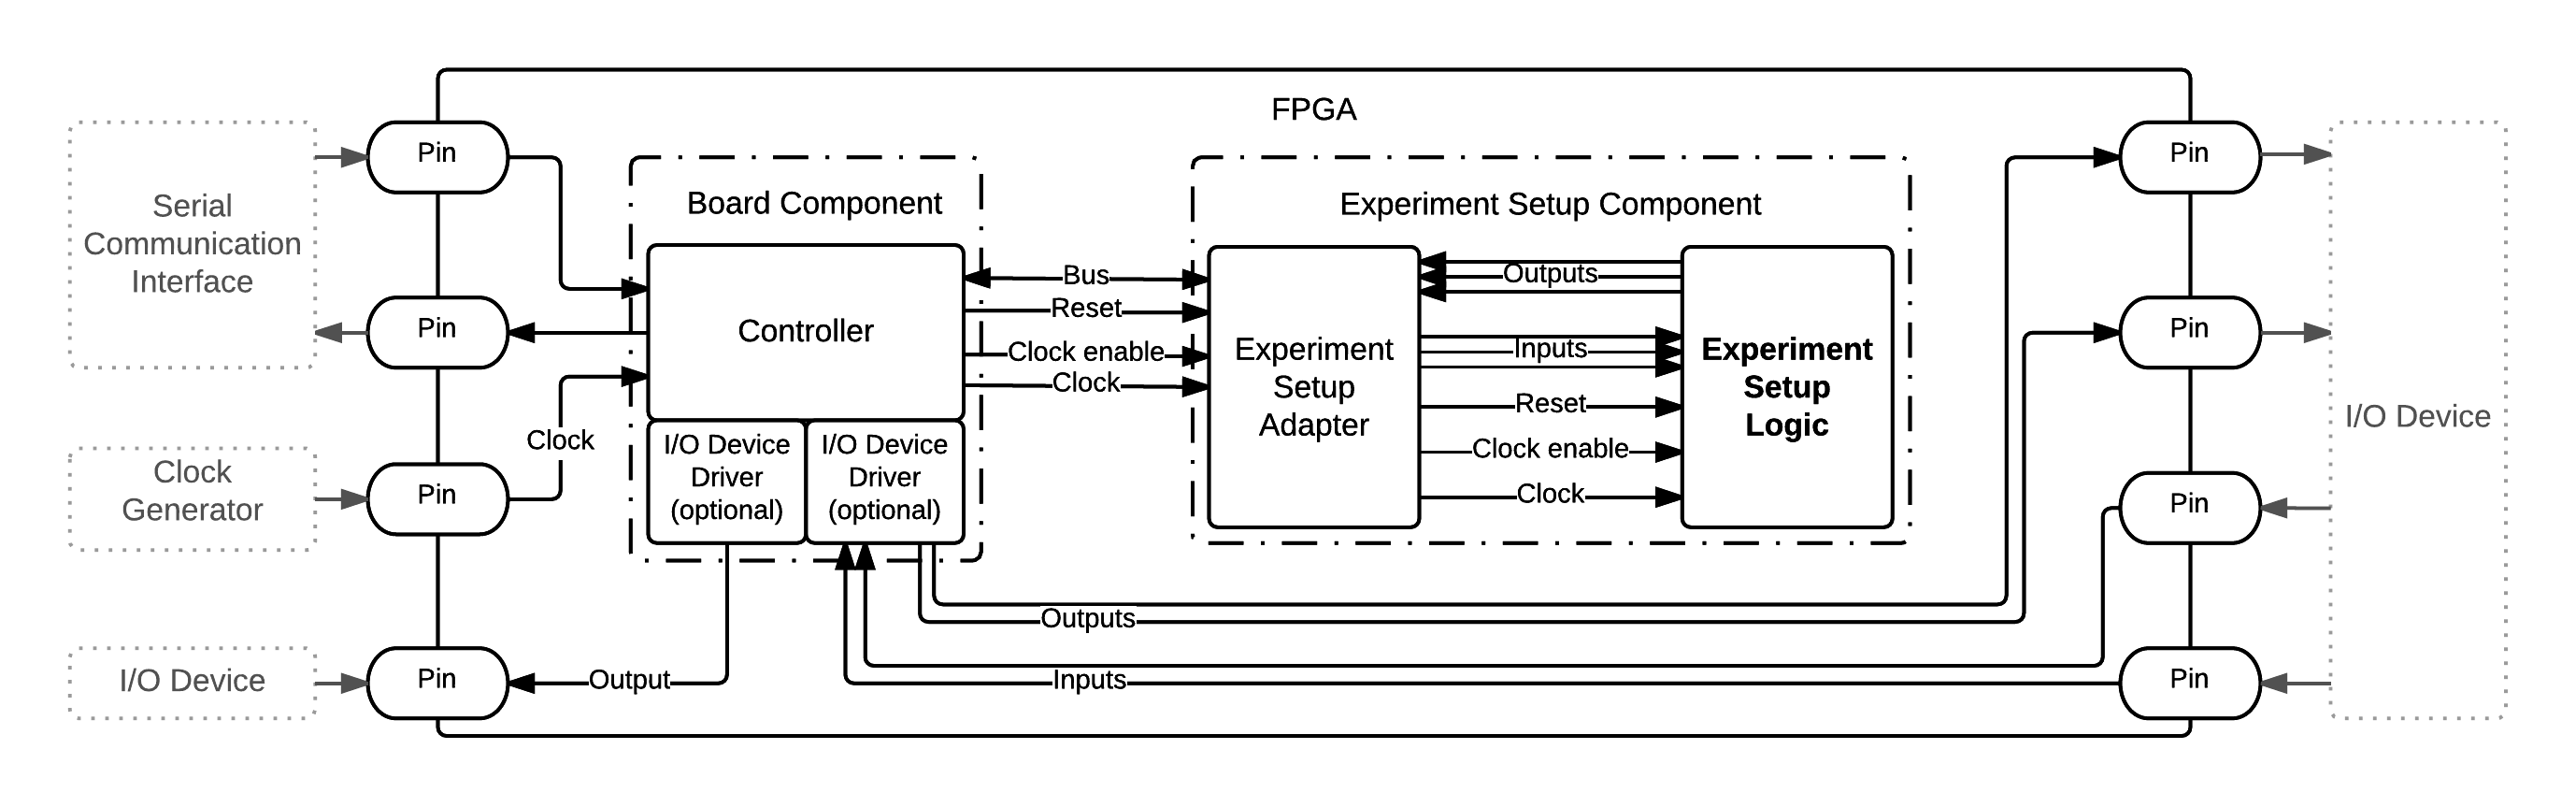
\includegraphics[width=\textwidth]{img/fpga-io2}
% \end{figure}

% \begin{figure}
% \centering
% 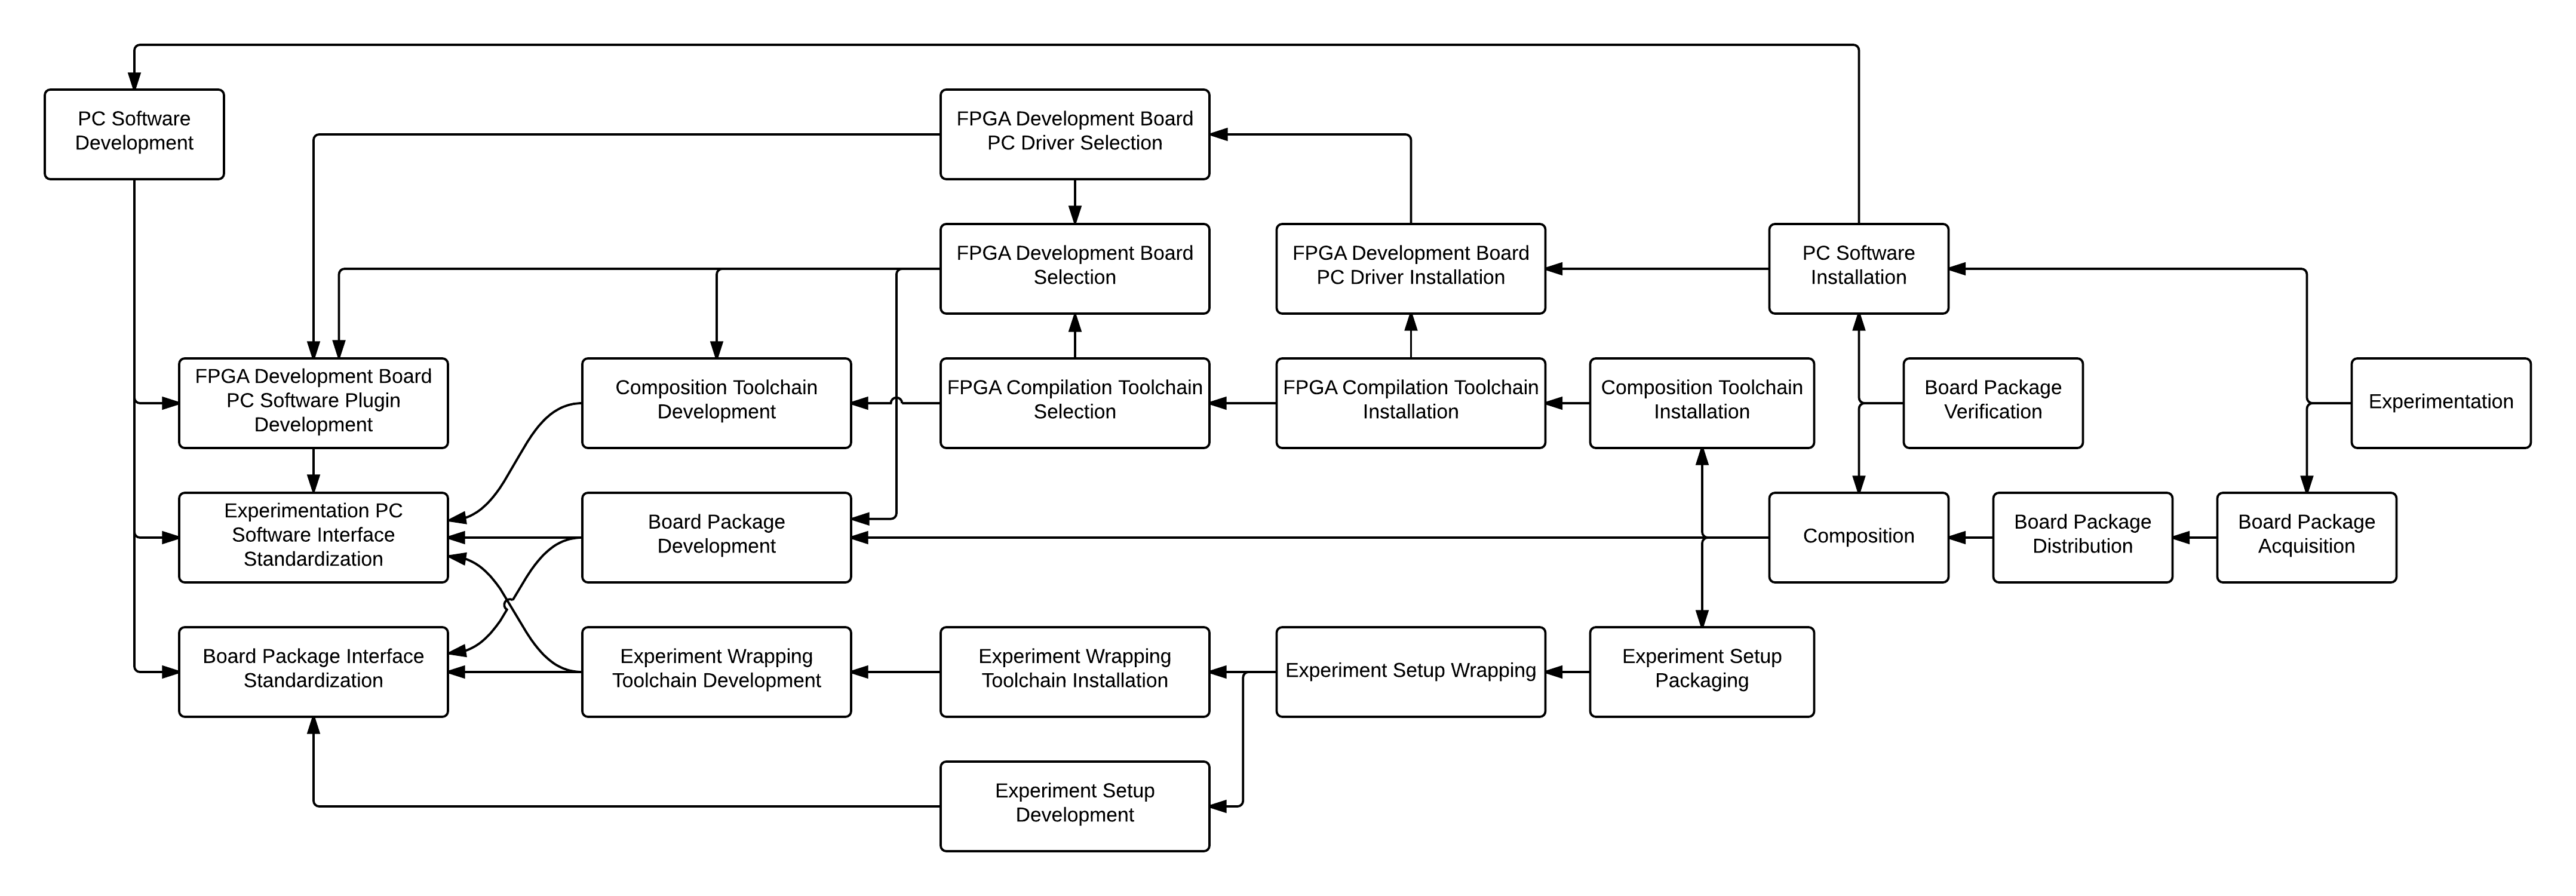
\includegraphics[width=\textwidth]{processes-dependencies-io}
% \caption{I/O reintroduced, Process dependency graph}
% \label{fig:processes-dependencies}
% \end{figure}

% \begin{figure}
% \centering
% \makebox[\textwidth][c]{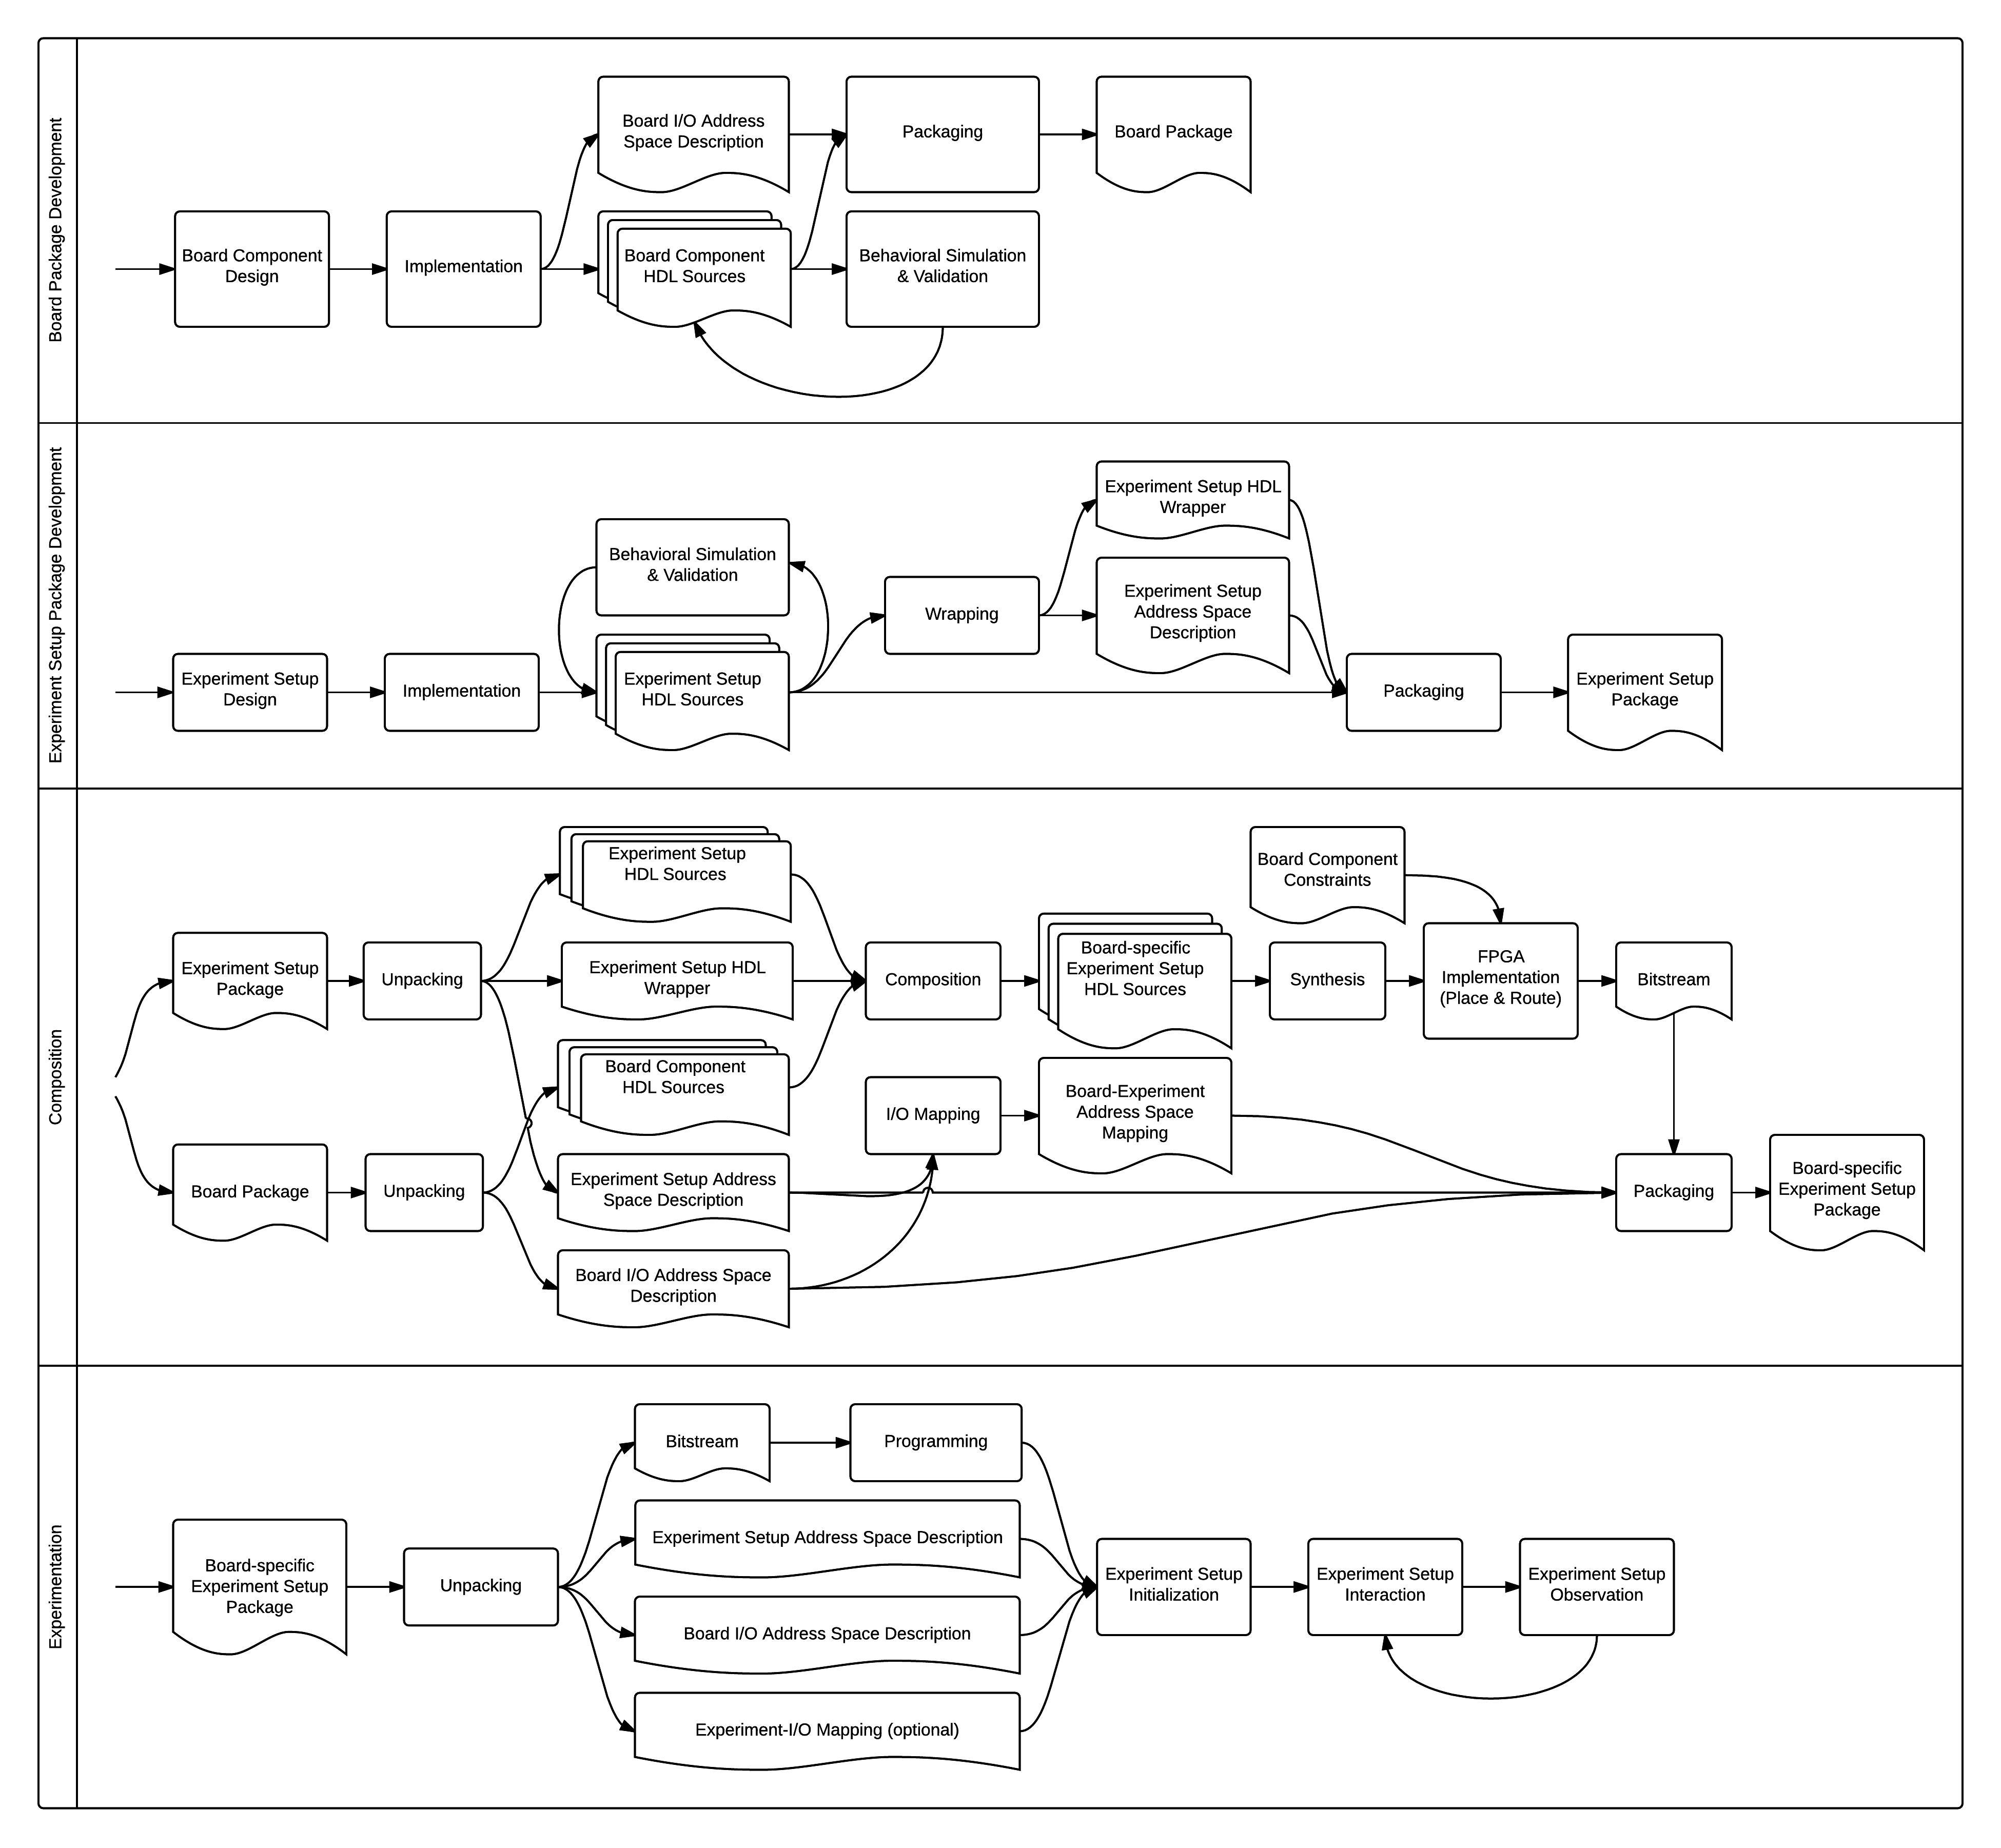
\includegraphics[width=1.25\textwidth]{processes-io}}
% \caption{I/O reintroduced, Processes overview}
% \label{fig:processes-io}
% \end{figure}

% \section{Student Requirements}
% A FPGA development board is connected to a student's PC. Two issues need to be addressed: an easy way of programming the FPGA in order to setup the experiment and communication with the FPGA to allow for interaction during the experiment. 

% Manufacturer development tools often facilitate these functions.

% They install FPGA board operating system drivers and experiment host software. An experiment is prepared by the course instructors and distributed to students. By loading the experiment, the fpga should be automatically programmed. The FPGA is not reprogrammed during the experiment. The student only interacts with the experiment through the experiment host software or the physical board as if it were the experiment hardware itself. 

% \section{Instructor requirements}
% It should be easy for instructors to create, test and distribute experiments. For the development of these experiments, instructors should be able to make use of existing development tools. 

% \section{Conceptual Model}
% In combinatorial logic, the output of signals is not dependent on the state of the digital circuit. In sequential logic, the output is dependent on the input signal levels, as well as the levels of previous input signals, the state of the circuit. Sequential logic is usually synchronous, meaning that state changes are triggered by a clock signal. 

% The circuit's state needs to be transfered to the student's PC such that it can be interpreted. 

% From an abstract point of view, a sequential circuit's state can be seen as a series of signals. Some signals are singular bit values, while others are composed of multiple bit values. Signals can be independent, while similar may be grouped by function, such as a set of cpu registers, data memory or instruction memory. 

% All these signals may be projected onto a memory space in order to allow for all signals of an experiment setup to be represented uniformly. 

% A file combined with the fpga program instructs the PC software on how to the memory space should be interpreted. This file is specific for one single version an FPGA program, but the same accross different FPGA board and desktop tools. In the fpga program it is determined how the experiment's signals are mapped onto the memory space. The PC software interprets these signals. 

% A fpga program may support multiple types of communication, such as serial rs232, ehternet, pci express etc...

% A distributable is specific for a combination of a FPGA development board model, a version of the FPGA program and a version of the PC tools. 

% The pc software must allow for the loading of a distributable, programming the experiment onto the FPGA and establishing a connection such that it can control the experiment. The PC software interprets the memory map of the fpga program and adapts its interface. After establishing a connection, the student can start the experiment by manually stepping a clock cycle, or set the clock cycle to increase automatically at a defined frequency. 


\end{document}